\documentclass[prd,amsfonts,onecolumn,superscriptaddress,aps,nofootinbib,11pt]{revtex4-1}

%\usepackage[top=3cm,bottom=3cm,left=2cm,right=2cm,marginparwidth=1.75cm]{geometry}
%\usepackage[utf8x]{inputenc} %LuaLaTeX
%\usepackage[T1]{fontenc}
%\usepackage[portuguese]{babel}
\usepackage{booktabs}
%comandos para linguagem especial 
\usepackage{amsmath, amsthm, amssymb, amsfonts, mathrsfs}
\usepackage{scalefnt}
\usepackage{physics, braket, slashed, bm}
\usepackage{bbold}
\usepackage{listings}
\usepackage{siunitx}
\usepackage{booktabs}
\usepackage{soul}
%\usepackage{icomma}
\usepackage{color}
\usepackage[usenames,dvipsnames]{xcolor}
%comandos para imagens, tabelas e legendas
\usepackage{graphicx}
%\usepackage[outdir=./]{epstopdf}
\usepackage{float}
\usepackage{placeins}
\usepackage{booktabs}
%comandos para hyperlinks
%\usepackage[strings]{underscore} %LuaLaTeX
\usepackage{hyperref}
\usepackage[compat=1.1.0]{tikz-feynman}
%\usepackage{subcaption}
%\usepackage{amssymb,amsmath}
%\usepackage{subfig}
%\usepackage{listings}
%\usepackage{caption}
%\usepackage{caption}
%\usepackage{subcaption}
\usepackage[caption=false]{subfig}
\usepackage{soul}
\usepackage{ulem}
\def\ds{\partial\!\!\!/}
\def\As{A\!\!\!/}
\def\Bs{B\!\!\!/}
\def\Ds{D\!\!\!/}
\def\bs{b\!\!\!/}
\def\ks{k\!\!\!/}
\def\ps{p\!\!\!/}


\hypersetup{
	% bookmarks=true,         % show bookmarks bar?
	unicode=false,          % non-Latin characters in Acrobat’s bookmarks
	pdftoolbar=true,        % show Acrobat’s toolbar?
	pdfmenubar=true,        % show Acrobat’s menu?
	pdffitwindow=false,     % window fit to page when opened
	%pdfstartview={FitH},    % fits the width of the page to the window
	pdfauthor={William},     % author
	colorlinks=true,       % false: boxed links; true: colored links
	linkcolor=blue,          % color of internal links
	citecolor=magenta,        % color of links to bibliography
	urlcolor=blue
}


%\providecommand{\be}{ \begin{equation} }
	%\providecommand{\ee}{\end{equation}}
%\providecommand{\bea}{\begin{eqnarray}}
	%\providecommand{\eea}{\end{eqnarray}}
%\providecommand{\nn}{\nonumber}
%\providecommand{\ol}{\overline}

\newcommand{\ad}[1]{{\color{blue}  #1}}

\DeclareMathOperator{\sign}{sign}

\renewcommand{\figurename}{Figure}
\renewcommand{\tablename}{Table}
%\renewcommand{\equationname}{Eq.}


\begin{document}
	
%\title{Probing Heavy Axion-Like Particles with Flavor Changing Interactions }
\title{ %Same-Sign Taus Signatures of Heavy Flavor Violating ALPs Scalars at the LHC \\ 
Same-Sign Taus Signatures of Maximally Flavor-Violating Scalars at the LHC }

\author{Alexandre Alves}
\email{aalves@unifesp.br}
\affiliation{Departamento de F\'isica, Universidade Federal de S\~ao Paulo, UNIFESP, 09972-270, Diadema, S\~ao Paulo, Brazil}
\author{Alex G. Dias}
\email{alex.dias@ufabc.edu.br}
\affiliation{Centro de Ci\^encias Naturais e Humanas, Universidade Federal do ABC,\\
09210-580, Santo Andr\'e-SP, Brazil}
\author{Eduardo da Silva Almeida}
\email{eduardo.silva.almeida.hep@gmail.com}
\affiliation{Centro de Ci\^encias Naturais e Humanas, Universidade Federal do ABC,\\
09210-580, Santo Andr\'e-SP, Brazil}
\author{Diego S. V. Gon\c{c}alves}
\email{diego.vieira@ufabc.edu.br}
\affiliation{Centro de Ci\^encias Naturais e Humanas, Universidade Federal do ABC,\\
09210-580, Santo Andr\'e-SP, Brazil}

\date{\today}
	
\begin{abstract}
We explore single and double flavor-violating scalars (flavons) production at the 13 and 14 TeV LHC in an effective field theory formulation where flavons always change the flavor of Standard Model fermions. When those scalars couple to mass, their flavor-changing couplings to top quarks and tau leptons are favored. Focusing on the mass region below the top quark mass, we find couplings that fit the muon and electron $(g-2)$ discrepancies and avoid several current experimental constraints. We determine the potential of the LHC to exclude or discover such a new physics scenario with clean signatures consisting of same-sign tau leptons and the simultaneous observation of resonances in the tau plus electron or muon invariant mass. We found that in the double production mode, effective couplings down to order $10^{-2}$ TeV$^{-1}$ can be probed for flavon masses in the 10-170 GeV range at the HL-LHC at 14 TeV, but couplings down to 0.1 TeV$^{-1}$ can be excluded at 95\% confidence level with data collected by the 13 TeV LHC in the same mass interval. 
\end{abstract}

\maketitle
	
\section{Introduction}


%Pseudo Nambu-Goldstone bosons like axions, which are related to a specific anomalous symmetry -- the Peccei-Quinn symmetry --, and axion-like particles (ALPs), related to general global symmetries~\cite{Jaeckel:2010ni,Ringwald:2012cu}, continue to receive great attention of the high energy physics community due to their testability and role in proposed solutions of problems left open by the Standard Model (SM). For the case in which these particles are very light and have feeble interactions,  there is a number of current and projected experiments aiming to scrutinize the parameter space of these as can be seen in Refs.~\cite{Workman:2022ynf,DiLuzio:2020wdo} and references therein. As it happens, due to their feeble couplings, these  particles cannot be probed at colliders. But, it may well be possible, especially for the ALP, that the new physics energy scale suppressing the interaction of these particles is low enough to be within the scope of the High-Luminosity LHC. Investigations of the production of such particles in colliders offer important complementary tests of their existence. We are going to deal with an ALP in this work.


%In fact, the LHC has been searching for the ALP in several production modes as photon fusion $\gamma \gamma \to a$ \cite{dEnterria:2013zqi, CidVidal:2018blh, Goncalves:2021pdc},  $Z$-boson decay $q \bar{q} \to \gamma^* \to a \gamma$, $q \bar{q} \to Z^* \to aZ$, and Higgs-boson decay $h \to aa$ \cite{CMS:2018nsh, CMS:2019spf, ATLAS:2020ahi, CMS:2020ffa, ATLAS:2021hbr}, $h \to aZ$ \cite{ATLAS:2020pcy}, as well as for several ALP decays modes as the decay of the ALP into photons $a \to \gamma \gamma$ \cite{dEnterria:2013zqi, CidVidal:2018blh, Goncalves:2021pdc}, leptons $a \to \mu^{+} \mu^{-}$ \cite{CMS:2018nsh, ATLAS:2020ahi, CMS:2020ffa, ATLAS:2021hbr}, $a \to \tau^{+} \tau^{-}$ \cite{CMS:2020ffa}, $a \to b \bar{b}$ \cite{CMS:2018nsh, CMS:2019spf, ATLAS:2021hbr} and so on.  Many constraints for ALP have resulted from these searches and future prospects are expected~\cite{dEnterria:2021ljz}. Previous phenomenological studies have anticipated  the viability of the searches like these and others, i.e involving SM particles and new neutrinos, for example, in final states at the LHC  ~\cite{Mimasu:2014nea,Brivio:2017ije,Bauer:2018uxu,Bauer:2017ris,Bauer:2017nlg,Jaeckel:2015jla,Alves:2016koo,Alves:2019xpc,Gavela:2019cmq,Merlo:2019anv,Baldenegro:2019whq,Dobrich:2015jyk,Harland-Lang:2019zur,Dobrich:2019dxc,Hahn:1404985,Alekhin:2015byh,Feng:2018pew,Aloni:2019ruo,Alves:2021puo,Knapen:2021elo,Alonso-Alvarez:2023wni,Cheung:2023nzg}. In all these developments, it is assumed that the ALP couplings to the SM particles conserve flavor.  

%Our aim in this work is to explore the hypothesis that the dominant ALP interactions violate flavor. It may be that the lack of ALP signals might be that the experimental devices and strategies are designed to search for the wrong types of ALPs. If those particles do not couple diagonally in the theory's flavor space but maximally violate the flavor conservation, then ALPs will not couple same-flavor bosons as well; that is, there will be no relevant couplings to photons, gluons, and electroweak gauge boson pairs. Of course, avoiding the hard constraints from flavor-changing neutral currents \textcolor{blue}{(FCNC) [...]} demands that flavor violation is predominantly a third-family effect, where ALPs couple to top quarks \textcolor{blue}{\st{and tau leptons}}. \textcolor{blue}{(Maybe, when we talk about FCNC we are talking about quarks. Even though our model has LFV, the word FCNC might refer specifically to quarks.)} On the basis of an Effective Theory, in which the ALP always \textcolor{blue}{changes} the flavor of SM fermions, we then study the single and double \textcolor{blue}{productions} and \textcolor{blue}{also the} decay of flavor-violating ALPs at the 14 TeV. These ALPs couple to mass, so that their flavor-changing couplings are more intense to top quarks and tau leptons. We just assume that the Effective Theory \st{is} originated from \textcolor{blue}{an} ultra-violet completed theory containing an approximated global symmetry whose spontaneous breaking an energy scale $v\simeq\Lambda$ \textcolor{blue}{gives} rise to the ALP.  

%We show that such ALP can be easily identified in proton-proton collisions at the LHC \st{if} \textcolor{blue}{when ("if" gives the impression that this is only possible in the regime $m_a < m_t$. We are also investigating the case when $m_a > m_t$ with some promising results!)} they are lighter than the top quark. \st{In this case,} \textcolor{blue}{Therefore, the largest branching ratio is when} the \st{ALPs decay} \textcolor{blue}{ALP decays} into tau plus an electron or muon. For the pair production, clean final states comprising hadronic same-sign taus, \textit{i.e.} $\tau^{\pm}_{\text{had}}\tau^{\pm}_{\text{had}}+\ell^\mp\ell^\mp$, with $\ell=e,\mu$, arise forming $\tau_{\text{had}}\ell$ resonances. We also explore the associated production of ALP plus a top quark, finding a \st{complementarity} between both search channels when systematic uncertainties are taken into account. \textcolor{blue}{(Complementarity might be an overstatement: When we inspect Figures \ref{fig:95cl} and \ref{fig:5sigma}, we notice that the $pp \to aa$ process dominates most of the $m_a$ range. The greater the systematic error introduced, the more the double production dominates, except the higher tail of $m_a$.)} Additionally, it is demonstrated the regions in the Effective Theory parameter space that could explain the ($g-2$) discrepancies of the muon and electron magnetic moment and are allowed by the current experimental \textcolor{blue}{constraints} over the width of the top quark, lepton flavor violation decays of the muon, $\mu\rightarrow\,e\,\gamma$, and the tau, $\tau\rightarrow\,e\,\gamma$, $\tau\rightarrow \mu\,\gamma$.

%Scalars that change the flavor of SM fermions have been searched for at the LHC 13 TeV by the ATLAS Collaboration through the top quark pair production, with one of them decaying into a light quark plus a scalar \st{which then make a flavor-conserving decays into a botton anti-botton} \textcolor{blue}{that decays into a $b\bar{b}$ flavor-conserving} pair~\cite{ATLAS:2023mcc}. According the Collaboration, the new branching ratio for the top quark decay into such scalar plus an up (charm) quark has upper limits between 0.019$\%$ (0.018$\%$) and 0.062$\%$ (0.078$\%$) for masses of the scalar particle between 20 GeV and 160 GeV. Although the nature of the scalar and the process is different from our proposal, it gives us the LHC potential for testing flavor-violating mediated by scalar/pseudo-scalars. Theoretically, the production signals at LHC of such particles were studied in top decay quarks from top quark pair production~\cite{Bhattacharyya:2022umc}, gluon fusion and with a single top with decay modes into heavy quarks and leptons~\cite{Tsumura:2009yf}, in association with the $Z$ boson has been investigated theoretically in~\cite{Bhattacharyya:2022ciw}. Outside the colliders scope, light pseudo-scalars like that \st{has} \textcolor{blue}{have} been investigated in connection to limits on lepton flavor violations decay of leptons, mesons, discrepancies of the muon and electron anomalous magnetic momentum~\cite{Cornella:2019uxs,Bauer:2019gfk}, fermion hierarchical flavor structure via Froggatt-Nielsen mechanism, dark matter, baryon asymmetry, and mesons oscilations~\cite{Ema:2016ops, Bjorkeroth:2018dzu}.  

%\begin{enumerate}
%    \item \textcolor{red}{We compared the \st{detection} exclusion and discovery thresholds for both processes with varying \st{systematics} \textcolor{blue}{systematic errors} levels. \st{We noticed that if the systematic error levels are much greater than $5\%$, the $pp \to aa$ process becomes the most competitive for detection/discovery purposes} The $pp \to aa$ process is the most competitive in most of the $m_a$ range;}

%    \item \textcolor{red}{We scanned the LFV constants space for values that would give a region on the $m_a \times \Lambda$ parameter space that could: (1) have a region explaining the $(g-2)$ limits, (2) make this region escape the top quark and LFV constraints, and (3) make this region be inside the \st{detection} exclusion/discovery regions of the two processes studied in this work. We were able to find such values for the LFV constants in two cases: when the ALP is \st{axial} a pseudoscalar or \st{mixed} violates parity. We were not able to find a suitable set of constants for the vectorial ALP;}

%    \item \textcolor{red}{For a specific set of LFV couplings, we plotted the $m_a \times \Lambda$ parameter space that had a discoverable ALP, in terms of the previous paragraph, for almost any mass in the range 10-170 GeV. We also plotted the future sensitivity of this set of couplings to the future LFV constraints facilities and noticed that part of the parameter region where the ALP could live can be probed.}

%    \item \textcolor{red}{Finally, we plotted some leading tau kinetic variables and noticed that there is no simple orthogonal cut we could make to improve our results. However, the results could be improved using machine learning techniques.};
%\end{enumerate}




\setcounter{page}{1}

Spin-zero particles with flavor-violating (FV) interactions are predicted in several models motivated by unresolved questions in the Standard Model (SM). Examples of such particles include pseudoscalars in the form of Nambu-Goldstone bosons, like  familons, which are associated with a symmetry among fermion families~\cite{Wilczek:1982rv,Reiss:1982sq,Gelmini:1982zz,Feng:1997tn}; majorons, which arise from the breaking of lepton number symmetry in connection to neutrino masses~\cite{Mohapatra:1979ia,Chikashige:1980qk,Chikashige:1980ui,Gelmini:1980re}; axions, which are the pseudo Nambu-Goldstone bosons of an anomalous global chiral symmetry proposed to solve the strong CP problem \cite{Peccei:1977hh,Weinberg:1977ma,Wilczek:1977pj,Georgi:1986df}, and can also be relevant in astrophysics, cosmology and flavor physics~\cite{DiLuzio:2020wdo,Ema:2016ops,Bjorkeroth:2018dzu}; and axion-like particles (ALPs), which bear some similarities with axions~\cite{Jaeckel:2010ni,Ringwald:2012cu,Dias:2014osa,Bauer:2021mvw,Jho:2022snj}. It is still possible that these particles are linked to the flavor $U(1)_F$ symmetry based on the Froggatt-Nielsen mechanism~\cite{Froggatt:1978nt}, which furnishes an explanation to the fermion hierarchical flavor structure through effectively suppressed Yukawa couplings. In this case, axions and ALPs can be also be identified as flavons~\cite{Ema:2016ops,Bjorkeroth:2018dzu} -- particles resulting from the breaking of flavor symmetry. 

As a general feature, the fields associated with these pseudoscalar  particles  have derivative couplings to the matter fields due to the presence of the shift symmetry $a(x)\,\rightarrow\,a(x)+\mathrm{constant}$ for the pseudoscalar field $a(x)$, and interactions suppressed by the energy scale in which their related global symmetry is broken.   
For the case in which these particles are very light and with feeble interactions, there are several experiments looking for them, including  astrophysical studies,  focusing on their diagonal couplings with leptons and photons~\cite{Workman:2022ynf,DiLuzio:2020wdo}. In these cases, they cannot be probed directly by colliders. But, it may well be possible, especially for sorts of ALPs and flavons, that the new physics energy scale suppressing the interactions is low enough to allow us to test the production of that particles through the proton-proton collisions of the High-Luminosity LHC. In fact, ALPs have been searched at the LHC in several production and decay modes conserving flavor~\cite{dEnterria:2013zqi, CidVidal:2018blh, Goncalves:2021pdc,CMS:2018nsh, CMS:2019spf, ATLAS:2020ahi, CMS:2020ffa, ATLAS:2021hbr,ATLAS:2020pcy,dEnterria:2013zqi, CidVidal:2018blh, Goncalves:2021pdc,CMS:2018nsh, ATLAS:2020ahi, CMS:2020ffa, ATLAS:2021hbr,CMS:2020ffa,CMS:2018nsh, CMS:2019spf, ATLAS:2021hbr}, resulting in a variety of constraints~\cite{dEnterria:2021ljz}. Previous phenomenological studies have anticipated  the viability of these searches and others  involving SM particles and new neutrinos in final states at the LHC, for example~\cite{Mimasu:2014nea,Brivio:2017ije,Bauer:2018uxu,Bauer:2017ris,Bauer:2017nlg,Jaeckel:2015jla,Alves:2016koo,Alves:2019xpc,Gavela:2019cmq,Merlo:2019anv,Baldenegro:2019whq,Dobrich:2015jyk,Harland-Lang:2019zur,Dobrich:2019dxc,Hahn:1404985,Alekhin:2015byh,Feng:2018pew,Aloni:2019ruo,Alves:2021puo,Knapen:2021elo,Alonso-Alvarez:2023wni,Cheung:2023nzg}. 

In this work, we explore the hypothesis that the dominant interactions of that particles violate flavor. If they do not couple diagonally in the theory's flavor space but maximally violate the flavor-conservation, then there will be no coupling with same-flavor bosons as well; that is, there will be no relevant couplings to photons, gluons, and electroweak gauge boson pairs. We will generically denote these particles by {\it flavons}, independently of the symmetry they are related. Of course, avoiding the hard constraints from flavor-changing neutral currents demands that flavor violation is predominantly a third-family effect, where flavons couple to top quarks. 

On the basis of an Effective Field Theory (EFT), in which the flavons always change the flavor of SM fermions, we study their single and double production at the LHC with energy 13 and 14 TeV at the center of mass. These scalars couple to mass, so that their couplings are stronger with the top quark and the tau lepton. We just assume that the EFT originates from an ultra-violet completed theory containing an approximated global symmetry, whose spontaneous breaking of an energy scale $v\simeq\Lambda$ gives rise to the flavon. 

We show that flavons lighter than the top quark can be easily identified in proton-proton collisions at the LHC. In this mass range, the largest branching ratio is when the flavon decays into tau plus an electron or muon. For the pair production, $q\bar{q}^\prime\,\rightarrow aa$, clean final states comprising same-sign taus, \textit{i.e.} $\tau^{\pm}\tau^{\pm}+\ell^\mp\ell^\mp$, with $\ell=e,\mu$, arise forming $\tau^\pm\ell^\mp$ resonances. We also explore the associated production of flavon plus a top quark, $qg \,\rightarrow ta$, showing the discovery potential for both search channels when systematic uncertainties are considered. We find that double production presents larger sensitivity in most of the flavon mass range, but single production complements the search for masses close to the top mass. Also, the impact of flavons on lepton flavor violations (LFV) has been explored. Additionally, we identify regions of the EFT parameter space that respect unitarity bounds, explain the ($g-2$) discrepancies of the muon and electron magnetic moments, and are safe from the current experimental constraints over the width of the top quark, LFV decays of the muon, $\mu\rightarrow\,e\,\gamma$, and the tau, $\tau\rightarrow\,e\,\gamma$, $\tau\rightarrow \mu\,\gamma$. 

Scalars with flavor-changing interactions have been searched for at the LHC. For example, through the top quark pair production, with one of them decaying into a light quark plus a scalar that decays into a $b\bar{b}$ flavor-conserving pair~\cite{ATLAS:2023mcc}, and also in decays of the Higgs boson or additional Higgs bosons, into $e^\mp\mu^\pm$~\cite{CMS:2023pte} and $\tau^\pm\ell^\mp$~\cite{ATLAS:2019pmk}.  The production signals at LHC of such particles were studied in top decay quarks from top quark pair production~\cite{Carmona:2022jid,Bhattacharyya:2022umc}, gluon fusion and with a single top with decay modes into heavy quarks and leptons~\cite{Tsumura:2009yf}, in association with the $Z$ boson has been investigated in~\cite{Bhattacharyya:2022ciw}. Besides the collider phenomenology, there are also investigations in connection to limits on lepton flavor violation decays of leptons, mesons, discrepancies of the muon and electron anomalous magnetic momentum~\cite{Cornella:2019uxs,Bauer:2019gfk,Carmona:2021seb,Muong-2:2006rrc,Muong-2:2015xgu,Hanneke_2008,Hanneke:2010au}. 



Our work is organized as follows: in Sec.~\ref{sec:model} we present the Effective Model and its parameters, on which our analysis is done; in Sec.~\ref{exp-const} the experimental constraints over the ALP are discussed in detail; in Sec.~\ref{backs} we discuss the signal of process and the relevant backgrounds; we present our analysis in Sec.~\ref{sec:analysis} and the results in Sec.~\ref{sec:results}; our conclusions are given in Sec.~\ref{conclusao}.



\section{Effective Model of Maximally Violating Flavons}
\label{sec:model}

The dimension-five effective Lagrangian describing flavon field, $a$, interactions is given by \cite{Cornella:2019uxs} 
\begin{equation}
    \mathcal{L} = - \frac{\partial_\mu a}{\Lambda} \sum_{f, i, j} \overline{f_i} \gamma^\mu (v_{ij} - a_{ij}\gamma_5) f_j \,,
    \label{eq:Lf}
\end{equation}
%where the diagonal ALP couplings to fermions and the ALP couplings to gauge bosons are considered zero as hypothesis. 
where $\Lambda$ is the new physics scale, and the axial and vectorial coupling constants between $a$ and the SM fermion flavors $f_i$ and $f_j$ are, respectively, $a_{ij}$ and $v_{ij}$. Through the use of the equations of motion, we can derive from Eq.~\eqref{eq:Lf} the following interaction terms of the flavon with fermions 
\begin{equation}
\label{eq:LFV-lagrangian}
    \mathcal{L} \supset -i \frac{a}{\Lambda} \sum_{f, i, j} \overline{f_i} \left[ (m_j - m_i) v_{ij} +  (m_j + m_i) a_{ij} \gamma_5 \right] f_j \,.
\end{equation}
In this form, we see that depending on the coefficients $v_{ij}$ and $a_{ij}$, the major contribution for couplings of the same order comes from the third family of fermions. The Lagrangian in Eq.~(\ref{eq:Lf}) might come from a theory with a global $U(1)_F$ spontaneously broken flavor-symmetry  under which each fermion can carry a different charge, which leads to the FV interactions. Taking into account that $a$ is a pseudoscalar field, it can be seen that the FV couplings $v_{ij}$ imply violation of parity symmetry in Eqs.~(\ref{eq:Lf}) and (\ref{eq:LFV-lagrangian}). However, the CP symmetry is preserved if $v_{ij}$ and $a_{ij}$ are real. In Appendix \ref{app:couplings}, we show how one could obtain these couplings in a sort of Froggatt-Nielsen effective field theory. 

Diagonal fermion couplings induce interactions with photons, gluons, and SM weak bosons. All these interactions lead to several strong experimental constraints which must be avoided in the search for a viable model. Gauge boson couplings can be suppressed by assuming that the diagonal couplings to SM and new quarks and leptons are either absent from the UV complete theory or that the new particles are too heavy to compete with the non-diagonal SM fermions decays. In order to bypass those constraints, we turn off all the diagonal lepton and quark couplings to the flavon %to avoid the more stringent experimental constraints
\begin{equation}
a_{ii} = 0 \,, \quad i=\ell, q.
%    a_{ee} = a_{\mu\mu} = a_{\tau \tau} = a_{uu} = a_{cc} = a_{tt} = v_{uu} = v_{cc} = v_{tt} = 0 = v_{ee} = v_{\mu\mu} = v_{\tau \tau} \,,
\end{equation}
%\textcolor{red}{We will suppress the superscript $f=u,e$ whenever it is clear from the lower indices which kind of fermions we are referring to.}

To avoid large flavor changing neutral currents at tree level, we only allow couplings of the top quarks to up and down quarks. This way, the only non-zero parameters of our model are the following:
%\begin{eqnarray}
%&&    m_a, \Lambda,\; \hbox{ALP mass and new physics scale} \nonumber\\
%&& v_{tc}, a_{tc}, v_{tu}, a_{tu},\; \hbox{non-diagonal top-quark couplings} \nonumber \\
%&& v_{e\tau}, a_{e\tau}, v_{\mu\tau}, a_{\mu\tau}, v_{e\mu}, a_{e\mu},\; \hbox{non-diagonal lepton %couplings} .
%\end{eqnarray}
\begin{equation}
\left\{
    \begin{array}{cc}
m_a, \Lambda & \hbox{flavon mass and new physics scale} \\
v_{tc}, a_{tc}, v_{tu}, a_{tu} & \hbox{non-diagonal top-quark couplings} \\
v_{e\tau}, a_{e\tau}, v_{\mu\tau}, a_{\mu\tau}, v_{e\mu}, a_{e\mu} & \hbox{non-diagonal lepton couplings}
    \end{array}
    \right.
\end{equation}

In this work, we will restrict our analysis to flavons lighter than top quarks, with masses between 10 and 170 GeV\footnote{Maximaly-violating flavons heavier than the top quark will be discussed in a forthcoming work.}. As a consequence,  the flavon branching ratio is almost 100\% in taus plus an electron or muon and only a tiny fraction into electron-muon. Note that producing these scalars at hadron colliders is viable only through top-quark couplings. Because diagonal couplings to fermions are absent, effective couplings to all SM bosons are suppressed. Therefore, gluon fusion, weak boson fusion, and associated production with weak bosons are out of hand at hadron colliders.
%If we consider ALPs heavier than the top quark, all the branching ratios would be in top quarks with anti-up and anti-charm quarks, and the same for your antiparticles.

The Standard Model is a consistent theory and does not violate unitarity at high energies. However, when we add higher dimensional effective operators, the theory might predict scattering cross-sections that grow with the center-of-mass energy of the process violating the optical theorem at some point. For our Lagrangian, the strongest bounds from the $f_i \bar{f}_j \rightarrow f_i \bar{f}_j$ scattering are given by
%
\begin{equation}\label{eq:unitarity-bounds}
  \left|v_{ij} \right| < \sqrt{8\pi}\frac{\Lambda}{m_j\,-\,m_i} \;\;\mbox{and}\;\; \left|a_{ij} \right| < \sqrt{8\pi}\frac{\Lambda}{m_j\,+\,m_i}\, .
\end{equation}
The axial and vector couplings can be as large as $\left|v_{3i}\right|/\Lambda$, $\left|a_{3i}\right|/\Lambda \lesssim 1.4\times 10^{-2}(1.5)$ GeV$^{-1}$ in the case of top(tau) quark(lepton) couplings. These bounds differ somewhat from those of Ref.~\cite{Cornella:2019uxs} because, contrary to that work, we are assuming only non-diagonal couplings, see Appendix~\ref{appendix:unitarity}.

%{\color{red} Comentar estes vínculos.}



%<full lagrangian -> LFV-lagrangian -> turn-ff diagonal couplings>

%\begin{equation}
%    \mathcal{L} = - \frac{i a}{\Lambda} (\bar{u}\; \bar{c}\; \bar{t})\left(
%    \begin{array}{ccc}
 %   0 & v_{uc} & v_{ut} \\
 %   v_{uc} & 0 & v_{ct} \\
 %   v_{ut} & v_{ct} & 0 \\
 %   \end{array}
%    \right) \left(
%    \begin{array}{c}
%    u \\
 %   c \\
%    t \\
%    \end{array}
 %   \right)
%\end{equation}

%\begin{equation}
%    \begin{split}
%        \mathcal{L} = - \frac{i a}{\Lambda} \bigg[ & g_{e\mu}(m_\mu+m_e)\overline{e}\gamma_5\mu + g_{e\tau}(m_e+m_\tau)\overline{e}\gamma_5\tau  +  g_{\mu\tau}(m_\mu+m_\tau)\overline{\mu}\gamma_5\tau \\ + & g_{tc}(m_t+m_c)\overline{t}\gamma_5c + g_{tu}(m_t+m_u)\overline{t}\gamma_5u +  2g_{uu}m_u\overline{u}\gamma_5u + 2g_{cc}m_c \overline{c}\gamma_5c \\ + & 2g_{tt}m_\tau\overline{t}\gamma_5t + f_{e\mu}(m_\mu-m_e)\overline{e}\mu + f_{e\tau}(m_e-m_\tau)\overline{e}\tau \\ + & f_{\mu\tau}(m_\mu-m_\tau)\overline{\mu}\tau + f_{tc}(m_t-m_c)\overline{t}c + f_{tu}(m_t-m_u)\overline{t}u \bigg] \,.
 %   \end{split}
%\end{equation}


\section{Experimental Constraints}
\label{exp-const}
 
 Besides the partial wave unitarity bounds, many experimental constraints apply. For the mass range we consider, we need to check the flavon contribution to the decay of top quarks, $Z$, and $W$ bosons and LFV-induced transitions. We list below the constraints considered in this work.

\begin{enumerate}
\item The measured model-independent top-quark decay width of $1.9 \pm 0.5$ GeV~\cite{ParticleDataGroup:2022pth} imposes an upper limit on the top quark-flavon coupling. The top quark partial width into $Wb$ is $1.322$ GeV at NNLO in QCD and it is measured to be $1.42$ GeV~\cite{ParticleDataGroup:2022pth}. Assuming the difference from this value to the experimental constraint is due to the new channels involving the new scalar, we impose the constraint
\begin{equation}
\Gamma(t\to a+u)+\Gamma(t\to a+c) < 0.5 \, \hbox{GeV}\, . 
\label{eq:br}
\end{equation}
The analytic expression for the width $t \to aq$, with $q = u,c$ is given in Appendix \ref{app:decay}. This constraint implies $\mathrm{BR}(t\to aq)<0.25$, $q=u,c$.

%We can find the exclusion region of $\Lambda$ in terms of $m_a$ as
%\begin{equation}
%	\frac{\Lambda}{c_{tq}} > \frac{(m_t^2 - m_a^2)}{\sqrt{16 \pi m_t %\Delta \Gamma_t}} \,,
%\end{equation}
%where we have neglected the light quark masses.

\begin{figure}[!ht]
    \centering
       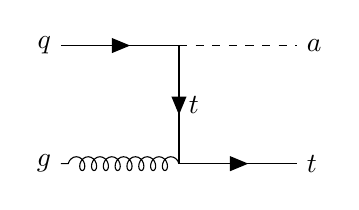
\begin{tikzpicture}[baseline=(current bounding box.center)]
    \begin{feynman}
        \vertex (a2);
        \vertex [right=of a2] (a3) {\(a\)};
        \vertex [left=of a2] (a1) {\(q\)};
        \vertex [below=of a2] (b2);
        \vertex [right=of b2] (b3) {\(t\)};
        \vertex [left=of b2] (b1) {\(g\)};
        \diagram* {
        (a1) -- [fermion] (a2) -- [fermion, edge label=\(t\)] (b2) -- [gluon] (b1),
        (a2) -- [scalar] (a3),
        (b2) -- [fermion] (b3)
        };
    \end{feynman}
\end{tikzpicture} 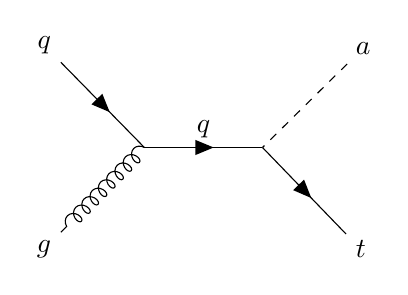
\begin{tikzpicture}[baseline=(current bounding box.center)]
    \begin{feynman}
        \vertex (b2);
        \vertex [above left=of b2] (a1) {\(q\)};
        \vertex [below left=of b2] (c1) {\(g\)};
        \vertex [right=of b2] (b3);
        \vertex [above right=of b3] (a4) {\(a\)};
        \vertex [below right=of b3] (c4) {\(t\)};
        \diagram* {
            (a1) -- [fermion] (b2) -- [gluon] (c1),
            (b2) -- [fermion, edge label=\(q\)] (b3),
            (a4) -- [scalar] (b3) -- [fermion] (c4),
        };
    \end{feynman}
\end{tikzpicture}  \begin{tikzpicture}[baseline=(current bounding box.center)]
    \begin{feynman}
        \vertex (a2);
        \vertex [right=of a2] (a3) {\(a\)};
        \vertex [left=of a2] (a1) {\(q\)};
        \vertex [below=of a2] (b2);
        \vertex [right=of b2] (b3) {\(a\)};
        \vertex [left=of b2] (b1) {\(\bar{q}^{\prime}\)};
        \diagram* {
        (a1) -- [fermion] (a2) -- [fermion, edge label=\(t\)] (b2) -- [fermion] (b1),
        (a2) -- [scalar] (a3),
        (b2) -- [scalar] (b3)
        };
    \end{feynman}
\end{tikzpicture}
    \caption{Feynman diagrams for single (left and central panels) and double (right panel) production of maximally flavor-violating scalars in hadron collisions. Single production is suppressed by $(m_t/\Lambda)^2$ while double production is suppressed by $(m_t/\Lambda)^4$.}
    \label{fig:prod}
\end{figure}

 \item The lepton-flavon coupling contributes to the $Z$ total decay width if its mass is such that $Z\to \tau+\ell+a$ is allowed. We checked that the new partial width is of order $10^{-11}$ GeV in the flavon mass range up to $m_Z-m_\tau$, thus much smaller than the $Z$ boson width uncertainty of $10^{-3}$ GeV~\cite{2006257}. We also checked that the impact of flavons on the $W$ boson width~\cite{https://doi.org/10.48550/arxiv.1012.2367} is negligible.
 
 %The Z boson decays into $a$ if $m_a < m_Z = 91.2 \, \si{GeV}$,  in order to avoid the constraint imposed by the experimental value of $\Gamma_Z$ \cite{2006}, this new partial width cannot exceed the uncertainty of order $10^{-3} \, \si{GeV}$. Our model is safe from such constraint since the new decay channel is lower than $10^{-11} \, \si{GeV}$ for $20 \, \si{GeV} < m_a < 80 \, \si{GeV}$. The same argument holds for the decay of $W$ boson to ALP  \cite{https://doi.org/10.48550/arxiv.1012.2367}.

 

 \item It is also necessary to check if the flavon decays fast enough for its by-products to be found inside the detector. For the mass range and couplings of interest in this work, we found that the flavon decays promptly after its production well inside the inner tracking region of the detector.
 %Supposing that, after its production, the ALP is traveling at speeds close to the light, we can calculate the mean distance it will travel as a function of its mass. This expression will be given by
 %\begin{equation}
 %    d [\si{m}] = \gamma c [\si{m s^{-1}}] \times \tau_a [\si{GeV^{-1}}]  \times 6.582 \times 10^{-25} \frac{\si{s}}{\si{GeV^{-1}}}\,,
 %\end{equation}
%where $\tau_a = 1/\Gamma_a$ is the mean lifetime of $a$, as calculated numerically by \texttt{MadGraph5\_aMC@NLO}. Figure (\ref{fig:distance}) shows that the average distance traveled by the ALP is very small compared to the dimensions of the detector, $\sim 1 \, \si{m}$.

%\begin{figure}
%    \centering
%    \includegraphics[scale=0.5]{pics/distance.pdf}
%    \caption{Average distance traveled by the ALP after its generation. Distances below $1 \, \si{m}$ imply that the ALP safely decays inside the detector. The Lorentz factor used in this figure is $\gamma = 1399.9999999767624$.}
%    \label{fig:distance}
%\end{figure}


\item The most stringent constraint comes from the MEG experiment of muon decay to electron and photon \cite{https://doi.org/10.48550/arxiv.1605.05081}. Following the null results,  the limits on the branching ratio of the muon in this channel is of order $10^{-13}$. The planned MEG II is expected to improve that limit by an order of magnitude. The BABAR collaboration, by its turn, searched for this LFV process in the tau-channel, the limits in $\tau \rightarrow e \gamma$ and $\tau \rightarrow \mu\gamma$ are of order $10^{-8}$ \cite{BaBar:2009hkt}. 

\end{enumerate}



\section{Signal and Background Simulations}\label{backs}

We simulated signals and backgrounds in leading order at the 13 and 14 TeV LHC with \texttt{MadGraph5}~\cite{Alwall:2014hca, Frederix:2018nkq} using the \texttt{UFO}~\cite{Degrande:2011ua} files generated by \texttt{FeynRules}~\cite{Alloul:2013bka} where we implemented our effective model.  The parton shower and detector simulations were performed in the default settings of \texttt{PYTHIA 8.3} \cite{Bierlich:2022pfr} and \texttt{Delphes3}~\cite{deFavereau:2013fsa}, respectively. The signal we consider comprises simple and double flavon productions in Figure~\ref{fig:prod}. The branching ratio of the flavon to $\tau+\ell$ is nearly 100 \% if $m_a<m_t$, as discussed earlier. The signal events were simulated setting $c_{tu}=c_{tc}=1$ and $\Lambda=1$ TeV. As the signals are proportional to powers of $c_{tq} m_t/\Lambda$, we rescale our cross sections for a given fixed flavon mass in our analyses. We employed the \texttt{NN23LO1} PDF set~\cite{Ball_2017} in all simulations. In order to estimate the impact of higher order QCD corrections, we simulate signals and backgrounds with up to two extra jets in the MLM merging approach~\cite{Mangano_2007}.

%\begin{figure}
%    \centering
%    \includegraphics[scale=0.55]{pics/BR_top_alp.pdf}
%    \caption{The branching ratio BR$(t \to aq)$ for various values of ALP masses as a function of the cutoff scale, $\Lambda$. The shaded area represents the constraint from Eq.~\eqref{eq:br}.}
%    \label{fig:BR_top_alp}
%\end{figure}


%furthermore we can search for final states with taus of the same sign, as an consequence we only have reducible background for this process. The disadvantage of this channels is that we lose sensitivity in couplings of the ALPs to leptons because of the branching ratio, but we gain in the cross-section and of course a better significance.


The main production modes of maximally-violating flavons are double and single production.
The double production
\begin{equation}
    q\bar{q}^\prime \to aa\; ,
\end{equation}
where $q(q^\prime)=u,c$ with a top quark exchanged in the $t$-channel, is suppressed by $(m_t/\Lambda)^4$ but it is initiated by valence up quarks, see Figure \ref{fig:prod}, right panel. 

The single production where the flavon is produced in association with a top quark 
\begin{equation}
    qg\to at\; ,
\end{equation}
occurs via a $t$-channel diagram as well, as shown in Figure \ref{fig:prod}, left and central panels. In this case, however, the final state is heavier compared to $a+a$ due to the presence of a top quark, but its cross section is suppressed by $(m_t/\Lambda)^2$. We also take the $\bar{t}+a$ contribution in our analysis.

 We show, in Figure~\ref{fig:xsec-times-efficiency}, the production cross-section, in pb, for double (solid black line) and  single (dashed black line) production at the 14 TeV LHC. For masses up to $\sim 120$ GeV, the flavon pair production ($q\bar{q}^\prime$ channel) exceeds the single production ($qg$ channel), especially for lighter flavons. The combined effect of a lighter final state and two initial-state up quarks gives the double production an advantage even being suppressed by $(m_t/\Lambda)^4$. That advantage is lost as the flavons get heavy. The production cross section for both processes is larger than 1 pb for masses up to 120 GeV and drops to around 10 fb for $m_a\sim m_t$. These rates drop even further (red lines in Figure \ref{fig:xsec-times-efficiency}) as we impose selections and kinematic cuts on the final state particles as we discuss ahead.

%\begin{figure} %[ht!]
%    \centering
%    \includegraphics[scale=0.7]{pics/xsec.pdf}
 %   \caption{In the left panel, we plot the cross-section, in pb, for the channels $q\bar{q}$, $qg$, $gg$, $bg$, and $bq$.  In the right, we display the cross-section for the same channels after the basic cuts and selections are imposed. }
%    \label{fig:xsec}
%\end{figure}


\begin{figure}
    \centering
%    \includegraphics[scale=0.35]{pics/xsec_times_efficiency.pdf}
%    \includegraphics[scale=0.35]{pics/BR_top_alp.pdf}
    \includegraphics[scale=0.35]{pics/sigma_BR.pdf}
    \caption{The production cross section of flavon pairs ($\sigma_{qq}$) and associated flavon+top quark ($\sigma_{qg}$) at the 14 TeV LHC. The dashed lines depict the cross-section times selection efficiency as discussed in the text. The branching ratio BR$(t \to aq)$ for various values of flavon masses as a function of the cutoff scale, $\Lambda$. The shaded area represents the constraint from Eq.~\eqref{eq:br}.}
    \label{fig:xsec-times-efficiency}
\end{figure}

Due to the flavor violation, the double flavon production gives rise to same-sign $\tau$-leptons plus same-sign electrons/muons half the time. The taus decay to "one-prong" signatures with one charged particle around 85\% of the time, while "three-prong" decays with three charged particles occur at approximately 15\%. Total leptonic decays with one charged electron or muon have a branching ratio of 35.1\%, but leptonic decays make $\tau$-lepton identification more difficult. On the other hand, hadronic decays give rise to low multiplicity jets that can be more easily tagged as $\tau$-jets. Our strategy relies on the identification of charged $\tau$-leptons, so we propose a search for signals with hadronic taus 
\begin{equation}
q\bar{q}^\prime\to aa\to \tau_h^\pm\tau_h^\pm+\ell^\mp \ell^\mp,\; \ell=e,\mu\; .
\end{equation}
This is a very clean signature if we are able to reconstruct the $\tau$-leptons charges. Also, notice that the decay of taus yields neutrinos, then the signals involve missing energy as well.%That is possible for hadronic decays of tau leptons, where low multiplicity jets denounce the production of taus. %Note, however, that this production mode is suppressed by $(m_t/\Lambda)^4$.

In the case of associated flavon+top quark production,  if the top quark decays to a flavon plus an up or charm quark, the two flavons generate the same-sign tau pair again, but the $t\to aq$ branching is suppressed by $\Lambda$ as shown in Figure~\ref{fig:xsec-times-efficiency}. Instead, we look at the dominant channel where the top quark decays to $Wb$ and still select events with same-charge taus with one tau originating from the $W$-boson decay
\begin{equation}
    qg \to a t \to a+W b\to \tau_h^{\pm} \tau_h^{\pm} + \ell^{\mp} + \nu_\tau + b \;.
\end{equation}

We show, in Tables~\eqref{tab:double} and \eqref{tab:simple}, all the reducible and irreducible background sources considered in our work. Next, we discuss the phenomenological analysis of the work.

%The model-independent (that is, without assuming it decays to $Wb$ exclusively) total width of the top quark is currently measured to be $\Gamma_t^{(\text{ATLAS})} = 1.9 \pm 0.5$~\cite{atlas-top-width}. Assuming only the standard model, $BR(t\to Wb)=1$, we have  $\Gamma_t^{(\text{PDG})} = 1.42^{+0.19}_{-0.15}$~\cite{top-wb}. If we consider the difference between the mean value of both measurements is due to some unknown decay channel, such as $t \to aq$, we can set the upper limit on $\text{BR}(t \to aq)$ as $(\Gamma_t^{(\text{ATLAS})} - \Gamma_t^{(\text{PDG})})/ \Gamma_t^{(\text{ATLAS})} = 0.252631578947$. This limit excludes the lower end of the parameter $\Lambda$.

%To create this plot, we used the PDG value for the top decay width, $\Gamma_t^{(\text{PDG})} = 1.42^{+0.19}_{-0.15}$ and the model-independent value measured by the ATLAS collaboration, $\Gamma_t^{(\text{ATLAS})} = 1.9 \pm 0.5$. The PDG limit assumes the $t$-quark decays only into $Wb$. If we consider the difference between the mean value of both measurements as due from unknown decay channels, such as the $t \to aq$, we can set the upper limit on $\text{BR}(t \to aq)$ as $(\Gamma_t^{(\text{ATLAS})} - \Gamma_t^{(\text{PDG})})/ \Gamma_t^{(\text{ATLAS})} = 0.252631578947$. This limit excludes the lower end of the parameter $\Lambda$.

%There are possible backgrounds coming from $t \bar{t}$ processes, $t\bar{t}\to W^\pm W^\mp b\bar{b}\to \tau^\pm \ell^\mp + b\bar{b}+\nu\nu$, $t\bar{t}\to W^\pm W^\mp b\bar{b}\to \tau^\pm \tau^\mp + b\bar{b}+\nu\nu$, and from single top processes $tW^\pm \to W^\mp W^\pm+b\to \tau^\pm \ell^\mp + b+ \nu\nu$ and $tW^\pm \to W^\mp W^\pm+b\to \tau^\pm \tau^\mp + b+ \nu\nu$. From double gauge boson production processes, $ZW^\pm  \to \tau^+\tau^- + \tau^\pm + \nu$, $ZW^\pm j \to \tau^+\tau^- + \tau^\pm + \nu + j$, $W^\pm W^\mp \to \tau^\pm + \ell^\mp + \nu\nu$, $W^\pm W^\mp j\to \tau^\pm + \ell^\mp + \nu\nu + j$, $W^\pm W^\mp \to \tau^\pm + \tau^\mp + \nu\nu$, $W^\pm W^\mp j\to \tau^\pm + \tau^\mp + \nu\nu + j$, and $W^\pm W^\pm j j \to \tau^\pm \tau^\pm + jj +\nu\nu$. We also expect contributions from triple gauge boson production processes, $W^\pm W^\mp W^\pm  \to \tau^\pm\tau^\pm + \ell^\mp + \nu\nu\nu$, $W^\pm W^\mp W^\pm j \to \tau^\pm\tau^\pm + \ell^\mp + \nu\nu\nu + j$, and $Z Z W^\pm \to b \bar{b} + \tau^+ \tau^- + \ell^{\pm} \nu$. $Z$-jet is also possible $Z j \to \tau^{+}\tau^{-}j$. %
%where $\ell = \mu,e$. 




\begin{table} %[ht!]
\scalefont{1}

\begin{tabular}{c c}
\hline
Background & $\sigma_{\text{basic}}$ (fb) \\ 
\hline\hline%& $\sigma$ (fb) & Events  & $n$ \\ \hline \hline 

$t\bar{t}\to W^\pm W^\mp b\bar{b}\to \tau^{\pm}_h \ell^{\mp} + b\bar{b}+\nu\nu$ & $<0.5366$ \\ 
\hline %& $2.683 \times 10^4$ & $50000$ & $0$ \\ \hline\hline

$tW^\pm \to W^\mp W^\pm+b\to \tau^{\pm}_h \ell^{\mp} + b+ \nu\nu$ & $<0.0604$ \\ 
\hline %& $3.020 \times 10^3$ & $50000$ & $0$ \\ \hline \hline

$W^\pm W^\mp\to \tau_h^\pm + \ell^\mp + \nu\nu$ & $<0.06694$   \\  %& $3.347 \times 10^3$ & $50000$ & $0$ \\ \hline

$ZZ\to \tau_h^\pm\tau_{\ell}^\mp + \ell^\pm\ell^\mp$ & $0.0037$    \\ %& $46.38$ & $50000$ & $4$ \\ \hline

$ZZ \to 4\tau \to \tau_h^\pm \tau_\ell^\pm \tau_h^\mp \tau_\ell^\mp + 4 \nu$  & $5.4 \times 10^{-21}$\\
$ZW^\pm \to \tau^+ \tau^- + \ell^\pm + \nu$ & $0.012$ \\  
%& $198.5$ & $50000$ & $3$ \\ \hline
$ZW^\pm\to \ell^+\ell^- + \tau_h^\pm + \nu$  & $<0.003978$ \\ 
\hline  %& $1.989 \times 10^2$ & $50000$ & $0$ \\ \hline \hline


$W^+W^-Z(\gamma^*)\to \tau^+\tau^{-}\tau^{\pm}_{h}\tau^\mp_\ell + \nu\nu$  & $8.5 \times 10^{-4}$ \\  %& $1.526 \times^{-1}$  & $50000$ & $275$ \\ \hline
%\begin{tabular}[c]{@{}c@{}}$W^+W^-\gamma^*\to \tau^{\pm}_{\text{had}}\tau^{\mp}_{\text{had}}\tau^{\pm}_{\text{had}} + \ell^\mp + \nu\nu $\end{tabular}                                    & $5.4 \times 10^{-5}$    \\ \hline %& $1.802 \times 10^{-1}$               & $50000$ & $15$      \\ \hline\hline
\begin{tabular}[c]{@{}c@{}}$W^\pm W^\mp W^\pm \to \tau^{\pm}_h\tau^{\pm}_h + \ell^\mp + \nu\nu\nu $\end{tabular}                                                         & $<6.7 \times 10^{-7}$           \\  %& $3.333 \times^{-1}$               & $50000$ & $0$                \\ \hline
\begin{tabular}[c]{@{}c@{}}$W^+W^-Z\to \tau^{\pm}_h\tau^{\mp}_\ell\tau^{\pm}_h + \ell^\mp + \nu\nu $\end{tabular}   & $7.4 \times 10^{-11}$    \\  %& $7.889 \times 10^{-9}$ & $50000$ & $472$   \\ \hline
$W^+W^-\gamma^*\to \tau^{\pm}_h\tau^{\mp}_\ell\tau^{\pm}_h+ \ell^\mp + \nu\nu$                                    & $2.9 \times 10^{-7}$    \\ \hline %& $4.231 \times 10^{6}$  & $50000$ & $3405$    
total background & $< 0.684$ \\
\hline
\end{tabular}
\centering
\caption{Reducible and irreducible background cross sections, in fb, for the double production after the selection efficiencies at 14 TeV LHC. When a leptonic tau appears, it decays to $\tau^{\mp}_\ell\to \ell^\mp+\nu\nu$. Tau leptons without a subscript can be either of leptonic or hadronic type. In the last line of the table, we calculate the superior limit of the total background rate. This limit is taken to obtain the statistical significances after the cut on the tau-lepton mass as discussed in the text.}
\label{tab:double}
\end{table}




%The double production gives rise to two ALPs after the proton-proton collision. The ALPs decay into the same-sign tau pair afterward,the table bellow \eqref{tab:double} summarize the reducible backgrounds we considered, see
%\begin{equation}
%    p p \to a a \to \tau^{\pm} \tau^{\pm} \ell^{\mp} \ell^{\mp} \,.
%\end{equation}

%There are many processes that we can classify as backgrounds to this process. As in the previous case, we expect background events coming from $t \bar{t}$ and single top production processes, $t\bar{t}\to W^\pm W^\mp b\bar{b}\to \tau^{\pm}_{\text{had}} \ell^{\mp}_{\text{had}} + b\bar{b}+\nu\nu$ and $tW^\pm \to W^\mp W^\pm+b\to \tau^{\pm}_{\text{had}} \ell^{\mp}_{\text{had}} + b+ \nu\nu$. We analyzed the gauge boson pair production $W^\pm W^\mp\to \tau^\pm + \ell^\mp + \nu\nu$, $ZZ\to \tau^\pm\tau^\mp + \ell^\pm\ell^\mp$, $ZW^\pm \to \tau^+ \tau^- + \ell^\pm + \nu$ and $ZW^\pm\to \ell^+\ell^- + \tau^\pm + \nu$. Triple gauge boson production, with only hadronic taus, $W^+W^-Z\to \tau^{\pm}_{\text{had}}\tau^{\mp}_{\text{had}}\tau^{\pm}_{\text{had}} + \ell^\mp + \nu\nu$, $W^+W^-\gamma^*\to \tau^{\pm}_{\text{had}}\tau^{\mp}_{\text{had}}\tau^{\pm}_{\text{had}} + \ell^\mp + \nu\nu$, and $W^\pm W^\mp W^\pm \to \tau^{\pm}_{\text{had}}\tau^{\pm}_{\text{had}} + \ell^\mp + \nu\nu\nu$. We also looked for triple gauge boson production with hadronic and leptonic taus, $W^+W^-Z\to \tau^{\pm}_{\text{had}}\tau^\mp_{\text{lep}}\tau^{\pm}_{\text{had}} + \ell^\mp + \nu\nu$ and $W^+W^-\gamma^*\to \tau^{\pm}_{\text{had}}\tau^\mp_{\text{lep}}\tau^{\pm}_{\text{had}} + \ell^\mp + \nu\nu$, where, in both cases, the decay of the leptonic tau is $\tau^\mp_{\text{lep}} \to \ell^\mp+\nu\nu$. There are also processes with four gauge bosons, but their production rates are lower than 1 fb without taking dilution from branching ratios into account. None of the reducible background processes listed in Table \ref{tab:double} has a significant contribution, so we chose to neglect all of them.



\begin{table}[h!]

\scalefont{1}
\begin{tabular}{c c}
\hline
 Background & $\sigma_{\text{basic}}$ (fb) \\ \hline\hline 
 $t\bar{t}\to W^\pm W^\mp b\bar{b}\to \tau_{h}^\pm \ell^\mp + b\bar{b}+\nu\nu$ & $47.82$\\ %& $2.687 \times 10^4$ & $10^{6}$ & $1780$ \\ \hline
 
 $t\bar{t}\to W^\pm W^\mp b\bar{b}\to \tau_{h}^\pm \tau_{h}^\mp + b\bar{b}+\nu\nu$ & $4.88$ \\ 
 \hline%& $6.714 \times 10^3$ & $10^{6}$ & $727$ \\ \hline \hline

 $tW^\pm \to W^\mp W^\pm+b\to \tau_{h}^\pm \ell^\mp + b+ \nu\nu$ & $2.746$       \\ %& $3.018 \times 10^3$ & $10^{5}$ & $91$ \\ \hline
 $tW^\pm \to W^\mp W^\pm+b\to \tau_h^\pm \tau_{\ell}^\mp + b+ \nu\nu$ & $0.347$ \\ \hline%& $7.539 \times 10^2$ & $10^{5}$ & $46$ \\ \hline \hline
 
 $ZW^\pm(j)  \to \tau^+\tau^- + \tau_{h}^\pm + \nu$ & $0.02113$ \\ 
 %& $1.291 \times 10^2$ & $73313$  & $17$ \\ \hline

 $W^\pm W^\mp(j) \to \tau_h^\pm + \ell^\mp + \nu\nu$ & $0.1029$ \\ 
%& $3.803 \times 10^3$ & $73913$  & $2$ \\ \hline
 
 $W^\pm W^\mp(j) \to \tau_h^\pm + \tau_{\ell}^\mp + \nu\nu$ & $<0.0129$ \\ 
 \hline
 %& $9.545 \times 10^2$ & $74194$  & $0$ \\ \hline 
 
 %$W^\pm W^\pm j j \to \tau^\pm \tau^\pm + jj +\nu\nu$                                                                                                                               & $<4.1 \times 10^{-5}$         \\ \hline%& $4.093$                & $10^5$   & $0$                  \\ \hline\hline
 $W^\pm W^\mp W^\pm(j)  \to \tau_h^\pm\tau_h^\pm + \ell^\mp + \nu\nu\nu$ & $6.92\times 10^{-4}$  \\ %& $6.661 \times 10^{-1}$ & $10^{5}$ & $72$ \\ \hline
 
 $Z Z W^\pm \to b \bar{b} + \tau^+ \tau^- + \ell^{\pm} \nu$ & $1.14 \times 10^{-4}$ \\ 
 \hline%& $3.279 \times 10^{-2}$ & $10^{5}$ & $348$ \\ \hline \hline

 $Z j \to \tau_h^{\pm}\tau_{\ell}^{\mp}j$ & $<8.64$ \\ 
 \hline%& $8.648 \times 10^{5}$  & $10^{5}$ & 0 \\ \hline
 total background & $<64.58$ \\
 \hline
\end{tabular}
\caption{Background processes for the associate top+flavon production at the 14 TeV LHC. In the last line of the table, we calculate the superior limit of the total background rate. This limit is taken to obtain the statistical significances after the cut on the tau-lepton mass, as discussed in the text. Tau leptons without a subscript can be either of leptonic or hadronic type.}
\label{tab:simple}
\end{table}

\begin{figure}
    \centering
    \includegraphics[scale=0.35]{pics/cuts.pdf}
    \caption{In the left panel, we show the percentage of surviving events after successive final state selections in the associate $a+t$ production. In the right panel, the selection efficiencies for double production. In both cases, requiring two taus with the same charge has the biggest impact on the overall identification efficiency.}
    \label{fig:id}
\end{figure}



%\newpage

\section{Analysis}\label{sec:analysis}

We adopt two selection strategies, one for each production mode. The selection for double production demands two same-charge taus, and two same-charge electrons and/or muons but opposite to the taus charge.  For the single production, events must also contain two same-charge taus, one $\ell$ with the opposite charge to the taus, and one $b$-tagged jet.  In both cases, we also impose the following basic cuts %
\begin{eqnarray}
    && p_T^{\tau_h}  > 10 \, \si{GeV} \,, \left| \eta_{\tau_h} \right| < 2.5, \nonumber \\
    && p_T^{\ell}  > 10 \, \si{GeV} \,, \left| \eta_{\ell} \right| < 2.5, \nonumber \\
    && p_T^{j} >  30 \, \si{GeV} \,, \left| \eta_j \right| <  2.5, 
    \label{eq:basic_cuts}
\end{eqnarray}
where $\ell = e, \mu$ and $j$ denotes a $b$-tagged jet.

 The cross section times selection efficiency is shown in Figure~\ref{fig:xsec-times-efficiency} for the two flavon production modes. Overall, the efficiency of identifying two tau jets plus leptons and/or $b$-jets is low. With a fixed efficiency for a hadronic tau of 0.6, the \texttt{Delphes3}~\cite{deFavereau:2013fsa} default value, and taking the branching ratio of tau into hadrons as 0.65, we have an initial efficiency of $(0.65\times 0.6)^2=0.15$ for two hadronic taus. Taking into account minimal requirements for triggers, generation cuts, and identification of leptons, that efficiency drops further. However, we profit from almost vanishing background rates in these channels.

 Selecting same-sign taus and leptons is advantageous from the point of view of background contamination. In the SM, the dominant irreducible source for double production is $ZZ\to \tau_\ell^\pm\tau_h^\mp+\tau_\ell^\pm\tau_h^\mp$~, where two taus ($\tau_\ell$) decay leptonically and the other two ($\tau_h)$, hadronically.   The $\tau_h^\pm\tau_h^\pm+\ell^\mp\ell^\mp$ final state has been investigated in the scope of the 2HDM~\cite{Iguro:2019sly,Blanke:2022kpi} and the SM $ZZ\to 4\tau$ background was estimated to be negligible. However, many reducible background sources might contribute to backgrounds. We list in, Table~\ref{tab:double}, the background sources we consider in our analysis for the double flavon production and decay. The common feature of those background processes is the presence of additional leptons/$\tau$-jets from proton fragmentation and QCD radiation, which, combined with produced leptons/hadronic taus, might mimic the flavon pair signature. As anticipated in Refs.~\cite{Iguro:2019sly,Blanke:2022kpi}, the $ZZ$ background is negligible after selecting two same-sign taus and two same-sign leptons since the same-sign leptons originate from suppressed leptonic tau decays. On the other hand, we estimate that reducible backgrounds amount to approximately 0.7 fb, at most, with reducible $t\bar{t}$, $tW$, and $WW$ as the major contributions. As discussed in the next section, these backgrounds can further be suppressed by identifying the $\tau^\pm\ell^\mp$ peaks in their invariant mass distributions.

The background sources for single production are shown in Table~\ref{tab:simple}. In this case, we must also deal with $t\bar{t}$ and $tW$ production. However, as the final state of interest has just one charged electron/muon, contrary to the double production, the backgrounds pass the selection requirements more easily. Our estimate for the upper limit of the total cross section is much larger now, reaching around 65 fb. In Tables~\ref{tab:double} and \ref{tab:simple}, the inequalities indicate an upper limit estimate of the cross sections where no Monte Carlo events were found after imposing selections and basic cuts of Eq.~\eqref{eq:basic_cuts}.

We use the Asimov estimate for the statistical significance~\cite{Cowan_2011}
\begin{equation}
    Z(s, b, \sigma_b^2) = \sqrt{2 (s+b)\ln \frac{(s+b)(b+\sigma_b^2)}{b^2 + (s+b)\sigma_b^2} - 2 \frac{b^2}{\sigma_b^2} \ln \left(1 +\frac{s \sigma_b^2}{b^2 + b \sigma_b^2}\right)} \,,
\end{equation}
where $s$ and $b$, are the number of surviving signal and background events after the cuts are performed, and $\sigma_b^2 = \varepsilon_b b$ is uncertainty in the measure of $b$ as a function of the systematic uncertainty of the total background rate, $\varepsilon_b$. When no background events survive, we estimate the significance as $Z=\sqrt{s}$.

In Figure \ref{fig:id}, we depict the signal selection efficiency when we impose the sequential identification  of particle species. In the right panel, the identification of two same-sign tau jets in double production occurs in 10\% of the events with two identified same-sign electrons/muons in the 60-140 GeV mass range, approximately, but drops to only 1\% of $\ell^\pm\ell^\pm$ for $m_a<60$ GeV and flavon masses close to the top-quark mass. The maximum overall selection efficiency reaches $\sim 0.01$ for $m_a\sim 120$ GeV. In the case of associate flavon-top quark production, identifying events with at least one $b$-jet is efficient, and identifying at least one $b$-jet and one charged electron/muon reaches 20\% for heavier masses. However, as in the double production case, events with two additional tau jets of same-sign are much rarer. The overall identification efficiency also reaches 0.01 at most, but, different from the double production, the efficiency increases with the flavon mass towards the top mass. Despite the low signal identification efficiency, the impact on the backgrounds is much more severe, and choosing such a channel pays off.

In order to optimize the statistical significance even further, we impose a cut on the highest $p_T$ pair $\tau^\pm_h\ell^\mp$ mass, $M_{\tau\ell}$, determined by $|M_{\tau\ell}-m|\leq \delta m$, and performing a random search on $m_a$ and $\delta_m$ such that
\begin{equation}
    N_\sigma = \underset{m_a, \delta m}{\text{argmax}} \, Z(s(m_a, \delta m), b(m_a, \delta m), \varepsilon_b)\; . 
\end{equation}
Here $s(m_a,\delta m)$ and $b(m_a,\delta m)$ represent the number of signal and background events after the cut on the mass of the $\tau$-lepton pair for fixed $\varepsilon_b$. This cut turns the backgrounds to double production negligible and reduces the backgrounds to single flavon production by a factor of $\sim 0.25$ for lighter masses raising to no reduction at all for larger masses. We show, in Figure~\ref{fig:mtaulep},  the $\tau^\pm\ell^\mp$ mass for the double production process, after 139 fb$^{-1}$ of integrated luminosity at the 13 TeV LHC, in the cases where the flavon has masses of 80, 100, and 120 GeV and $c_{tq}/\Lambda=1$ TeV$^{-1}$ prior to the invariant mass cut. In the absence of backgrounds, these peaks should be easily identifiable, however, our reconstruction of the invariant mass is simplified compared to experimental analyses. For example, the search for LFV SM Higgs boson decays to $\tau^\pm\ell^\mp$~\cite{ATLAS:2019pmk} comprises multivariate tools to identify the various objects in final states with QCD and $\tau$-jets. Nonetheless, a reconstruction of the scalar resonance should be feasible within some degree of resolution.

%The lack of relevant backgrounds for the double production process lets us find the statistical significance of getting the square root of the signal which is given by
%\begin{equation}
%   Z = \sqrt{s}.
%\end{equation}
%Among the cuts we imposed, we can see in Figs. (\ref{fig:succesive-cuts}) and (\ref{fig:95cl-alp-15sys}) that the most penalizing is to require two taus with the same charge.
\begin{figure}
    \centering
    \includegraphics[scale=0.5]{pics/events_per_minv.pdf}
    \caption{The $\tau^\pm$-$\ell^\mp=e,\mu$ invariant mass for the double production $q \bar{q}^\prime \to aa$ for flavon masses of 80, 100, and 120 GeV. The histogram is normalized by the number of events expected at the 13 TeV LHC after 139 fb$^{-1}$. We estimate a negligible number of background events in this channel.}
    \label{fig:mtaulep}
\end{figure}

\section{Results}
\label{sec:results}

 We now present a sensitivity analysis for the potential of the 13 and 14 TeV LHC to exclude or discover the proposed signals of the model. 

 \subsection{Sensitivity of the LHC to top-quark couplings and flavon masses}
\begin{figure}[ht!]
        \centering
%        \begin{subfigure}[b]{0.475\textwidth}
%            \centering
%            \includegraphics[scale=0.4]{pics/95cl_alp_0sys.pdf}
%            \caption[Network2]%
%            {{\small 0\% systematics}}    
%            \label{fig:95cl-alp-0sys}
%        \end{subfigure}
%        \hfill
%        \begin{subfigure}[b]{0.475\textwidth}
%            \centering 
%            \includegraphics[scale=0.4]{pics/95cl_alp_5sys.pdf} \\
%            \caption[]%
%            {{\small 5\% systematics}}    
%            \label{fig:95cl-alp-5sys}
%        \end{subfigure}
%        \vskip\baselineskip
%        \begin{subfigure}[b]{0.475\textwidth}
%            \centering 
%            \includegraphics[scale=0.4]{pics/95cl_alp_10sys.pdf}
%            \caption[]%
%            {{\small 10\% systematics}}    
%            \label{fig:95cl-alp-10sys}
%        \end{subfigure}
%        \hfill
%        \begin{subfigure}[b]{0.475\textwidth}
%            \centering 
%            \includegraphics[scale=0.4]{pics/95cl_alp_15sys.pdf}
%            \caption[]%
%            {{\small 15\% systematics}}    
%            \label{fig:95cl-alp-15sys}
%        \end{subfigure}
        \includegraphics[scale=0.5]{pics/1.96.pdf}
        \caption{95\% C.L. exclusion region in the $m_a \times c_{tq}/ \Lambda$ parameter space. Red and black lines represent the $pp \to aa$ and $pp \to at$ processes, respectively. The solid and dashed lines represent the reach of these channels for $139 \, \si{fb^{-1}}$@13 TeV and $3000 \, \si{fb^{-1}}$@14 TeV limits, respectively. Each panel assumes a different level of systematic error. For systematic errors greater than $5\%$, the $pp \to aa$ process is the most competitive to exclude the model.}
        \label{fig:95cl}
    \end{figure}

Because the flavon decays almost exclusively into taus plus leptons, our analysis is not sensitive to lepton couplings since these parameters cancel out the branching ratios. Only the top-quark couplings $c_{tu}, c_{tc}$, and the flavon mass, $m_a$ can thus be probed. 

Figure \ref{fig:95cl} depicts the 95\% C.L. limits for both production channels. The confidence intervals take into account different levels of systematic errors. In all cases, sum over the quark contributions $q=u,c$ and fix $c_{tu}=c_{tc}\equiv c_{tq} =1$ in our simulations without loss of generality since the relevant parameter is the ratio $c_{tq}/\Lambda$. The red and black lines show the 95\% CL exclusion limits for the $pp \to aa$ and $pp \to at$ processes, respectively, and the shaded areas represent the excluded regions of the parameter space if no signal is observed. The solid and dashed lines represent the reach for integrated luminosities of $139 \, \si{fb^{-1}}$@13 TeV and $3000 \, \si{fb^{-1}}$@14 TeV, respectively. Double flavon production presents better prospects for exclusion in all systematic scenarios considered in this work. As shown in Figure \ref{fig:95cl}, the single production, which is contaminated by non-negligible backgrounds, is sensitive to systematic uncertainties. Yet, for flavon masses close to the top mass, single production wins over double production, complementing the exclusion limits. Moreover, note that limits from double production, where the statistical significance is just $\sqrt{s}$, scale as $L^{-1/4}$ with the luminosity and increasing data up to 3000 fb$^{-1}$ improves the sensitivity by a factor not much larger than 2.
%
\begin{figure}[ht]
        \centering
%        \begin{subfigure}[b]{0.475\textwidth}
%            \centering
%            \includegraphics[scale=0.4]{pics/5sigma_alp_0sys.pdf}
%            \caption[Network2]%
%            {{\small 0\% systematics}}    
%            \label{fig:5sigma-alp-0sys}
%        \end{subfigure}
%        \hfill
%        \begin{subfigure}[b]{0.475\textwidth}
%            \centering 
%            \includegraphics[scale=0.4]{pics/5sigma_alp_5sys.pdf} \\
%            \caption[]%
%            {{\small 5\% systematics}}    
%            \label{fig:5sigma-alp-5sys}
%        \end{subfigure}
        %\vskip\baselineskip
%        \begin{subfigure}[b]{0.475\textwidth}
%            \centering 
%            \includegraphics[scale=0.4]{pics/5sigma_alp_10sys.pdf}
%            \caption[]%
%            {{\small 10\% systematics}}    
%            \label{fig:5sigma-alp-10sys}
%        \end{subfigure}
%        \hfill
%        \begin{subfigure}[b]{0.475\textwidth}
%            \centering 
%            \includegraphics[scale=0.4]{pics/5sigma_alp_15sys.pdf}
%            \caption[]%
%            {{\small 15\% systematics}}    
%            \label{fig:5sigma-alp-15sys}
%        \end{subfigure}
        \includegraphics[scale=0.5]{pics/5.pdf}
        \caption{$5 \sigma$ discovery region in the $m_a \times c_{tq}/ \Lambda$ parameter space. Red and black lines represent the $pp \to aa$ and $pp \to at$ processes, respectively. The solid and dashed lines represent the reach of these channels for $139 \, \si{fb^{-1}}$@13 TeV and $3000 \, \si{fb^{-1}}$@14 TeV, respectively. Each panel assumes a different level of systematic error. For systematic errors in excess of $5\%$, the $pp \to aa$ process is the most competitive to discover a signal from this model.} 
        \label{fig:5sigma}
    \end{figure}

Fixing systematic errors on 5\%, effective coupling $c_{tq}/\Lambda$ of order $10^{-4}$($5\times 10^{-5}$) GeV$^{-1}$ can be excluded in double production for flavon masses around 80 GeV and integrated luminosity of 139 fb$^{-1}$@13 TeV (3000 fb$^{-1}$@14 TeV). Not observing single production events excludes $c_{tq}/\Lambda$ of order $10^{-3}$ for $150<m_a<170$ GeV irrespective the luminosity.
%The $pp \to at$ channel is competitive until we reach systematic errors of 5\% in the background rates, but for larger systematics, the $pp \to aa$ channel is better for exclusion.

The $5\sigma$ discovery regions for both channels are shown in Figure \ref{fig:5sigma}. We show the discovery potential for the current $139 \, \si{fb^{-1}}$@13 TeV (solid lines) and projected $3000 \, \si{fb^{-1}}$@14 TeV (dashed lines). Just like the 95\% CL limits, the discovery region from single flavon production depends on the systematic errors in the background predictions, and the single production becomes competitive $m_a$ closer to the top mass.

%In these figures, we also have set $c_{tq}=1$ and summed over the contribution of the quarks $q=u,c$. \st{Comparing these plots with the $95\%$ C.L. limits, we find that the $5\sigma$ discovery region is smaller, as one would expect.} 
%Nonetheless, the discovery threshold is competitive up to $5\%$ \st{systematics} \textcolor{blue}{systematic errors} scenario, like in the previous case. 
%\st{When systematics is the main source of errors, the $pp \to aa$ channel becomes the more competitive channel to search in the collision facility.} 

\subsection{Benchmarking model parameters}

 Now that we established the region of $c_{tq}/\Lambda$ {\it versus} $m_a$ that can be probed at the LHC, we look for lepton-flavon couplings that escape theoretical and experimental constraints but keep compatibility with the current muon and electron $(g-2)$ data. Our goal is to instantiate some model parameters to demonstrate their phenomenological viability. A thorough exploration of the parameter space might reveal other interesting spots but it is beyond the scope of this analysis.

%\st{Our next task is to solve the problem of finding values} Now we will find the values for the coupling constants that makes our model consistent with the current $(g-2)$ limits. \st{result in sensitivity for the $(g-2)$ constraints}. There is a \st{large} number of such couplings that generate reasonable solutions, so we need to sort them out.

Let us define $X = ( v_{e \mu}, v_{e \tau}, v_{\mu \tau}, a_{e \mu}, a_{e \tau}, a_{\mu \tau} )$ as a set of LFV couplings. We want to find elements of $X$ which are compatible with the $(g-2)_\mu$~\cite{Muong-2:2006rrc,Muong-2:2015xgu} and $(g-2)_e$~\cite{Hanneke_2008,Hanneke:2010au} data and lie inside the region of discovery of the LHC but evade the top decay constraint of Eq. (\ref{eq:top-decay}), the LFV-induced $\mu\to e\gamma$, $\tau\to e\gamma$, and $\tau\to \mu\gamma$  transitions of Eq. (\ref{eq:lfv-decay}), and the unitary bounds of Eq. (\ref{eq:unitarity-bounds}). 

The measured anomalous magnetic moment of the muon has been showing a longstanding discrepancy compared to the SM prediction of approximately $4\sigma$: $\Delta a_\mu = a_\mu^{\mathrm{exp}}-a_\mu^{\mathrm{SM}}=(27.1\pm 7.3)\times 10^{-10}$, while in the case of the electron, the discrepancy is around $2\sigma$: $\Delta a_e = a_e^{\mathrm{exp}}-a_e^{\mathrm{SM}}=(-87\pm 36)\times 10^{-14}$. To compute the contribution of the flavon to $(g-2)_\mu$ and $(g-2)_e$, we use the formulas (\ref{eq:g-2}), deduced in~\cite{Cornella:2019uxs}. 

%\textcolor{red}{The experimental values of the $(g-2)$ constraints are not changed by this analysis. Instead, we use closed-form solutions for $\Delta_{ae}$ and $\Delta_{a \mu}$ to see if a certain element of $X = ( v_{e \mu}, v_{e \tau}, v_{\mu \tau}, a_{e \mu}, a_{e \tau}, a_{\mu \tau} )$ lies inside of both uncertainty regions around $[\Delta_{ae} - \epsilon_{ae}, \Delta_{ae} + \epsilon_{ae}]$ and $[\Delta_{a\mu} - \epsilon_{a\mu}, \Delta_{a\mu} + \epsilon_{a\mu}]$. Thus, the so-called $(g-2)$ points are the pairs $(m_a, \Lambda)$ in the figure that when plugged inside the closed forms of $\Delta a_e$ and $\Delta a_\mu$ return a value that is inside the corresponding uncertainty region.}

To search for viable points, we take random samples of LFV couplings, the flavon mass $m_a$, and the new physics scale, $\Lambda$. Considering the decay rate equations in Appendix \ref{app:decay}, we performed a log-uniform scan in these parameters. The coupling constants were sampled from the interval $[10^{-3}, 2\times10^3]$, respecting the unitary bounds from Eq. (\ref{eq:unitarity-bounds}). Since we are interested in the flavon that is lighter than the top quark, the flavon mass was scanned in the range $[10, 170]$ GeV, while the new physics scale in the range $[1, 5000]$ GeV. We are also considering only points that satisfy $\Lambda > m_a$ to ensure the validity of the EFT approach in a minimum way.
%{\color{red} Há algum ponto para o qual $\Lambda < m_a$? Sim, mas não é muito relevant porque no final das contas devemos variar tanto $\Lambda$ e $m_a$ e verificar se a região azul é cortada pela linha $m_a = \Lambda$. Em nenhum dos casos que estamos analisando há este problemas. Vide os plots. Se for preciso, podemos adicionar a linha $m_a = \Lambda$ nos plots para ter certeza.} %Any set of such parameters was then expanded through the entire ranges of $m_a$ and $\Lambda$ keeping constant the couplings. The emerging region is composed of points $(m_a, \Lambda)$ compatible with the $(g-2)_\mu$ and $(g-2)_e$ data. 

%{\color{purple} Diego: explique melhor aqui, qual foi o range/distribuição considerado para massa dos flavons e $\Lambda$? }

Our analysis now focuses on the study of three cases: (I) purely vectorial, (II) purely axial, (III) and mixed couplings. In general, the constraints from $\mu\to e+\gamma$, $\tau\to e+\gamma$, and $\tau\to \mu+\gamma$, depend on the couplings of the lepton inside the loop amplitude with the external leptons and the new physics scale, $g_{ij}g_{ik}/\Lambda^2$, where $i$ is the flavor of the lepton inside the loop and $m_j>m_k$ must be respected in order the decay to be possible. This way, if we increase the couplings, the constraints extend to larger $\Lambda$, eventually excluding the points of the parameter space which are compatible with $(g-2)$ data and that can be discovered in the LHC.

\vskip0.5cm
\noindent{\underline{(I) Purely vectorial couplings, $v_{ij}\neq 0$}} 

Let us begin with the simplest cases of parity-conserving flavons, either purely scalar or purely pseudoscalar. For the scalar case, we set
\begin{equation}
    a_{e \mu} = a_{e \tau} = a_{\mu \tau} = 0 \,.
\end{equation}

We sampled one million points, but no solution evading constraints, explaining $(g-2)$, and that can be probed at the LHC was found. We conclude that a scalar flavon is strongly disfavored in the parameter space we consider here.

 \begin{figure}[h!]
    \centering
    \includegraphics[scale=0.5]{pics/g1.pdf}
    \caption{Purely axial flavon where $a_{e \tau} = a_{e \tau} = 0.1$ and varying $a_{\mu \tau}$. For $a_{\mu \tau} \approx 500$, solutions to $(g-2)$ avoid all constraints and lie inside the discovery region. Increasing $a_{\mu \tau}$
    pushes the points to weaker couplings, eventually dropping them from the LHC discovery region.}
    \label{fig:g1}
\end{figure}

\vskip0.5cm
\noindent{\underline{(II) Purely axial couplings, $a_{ij}\neq 0$}} 

In this case, we set all vectorial couplings to zero
\begin{equation}
    v_{e \mu} = v_{e \tau} = v_{\mu \tau} = 0 \,.
\end{equation}

 \begin{figure}[h!]
    \centering
    \includegraphics[scale=0.5]{pics/g2.pdf}
    \caption{Purely axial flavon where $a_{e \tau} = a_{e \tau} = 0.1$ and varying $a_{\mu \tau}$. We see that for higher values of $a_{e \tau} = a_{e \tau} = 0.1$ it becomes harder to find solutions without also increasing $a_{e \mu}$.}
    \label{fig:g2}
\end{figure}

Again, we sampled one million parameter settings, from which only 171 solutions were found. Analyzing these solutions, we investigated further the points described below %found some patterns shared among them. To simplify matters, we fix
\begin{equation}
    a_{e \tau} = a_{e \tau} = 0.1, \quad v_{e \mu}=v_{e \tau}=v_{\mu \tau}=0
\end{equation}
with $a_{e \mu}$ free to vary. In this case, we freeze the harder constraint from $\mathrm{BR}(\mu\to e+\gamma)$, which does not depend on $g_{e\mu}$ couplings but keeps control on $(\Delta a)_\mu$ and $(\Delta a)_e$ which do depend on those couplings.

In Figure \ref{fig:g1}, we show four scenarios: $a_{e\mu}=20,\; 300,\; 500,\; 2000$. First of all, notice that the blue points, the solutions to $(g-2)$, concentrate in the $m_a\gtrsim 100$ GeV region. The solutions for the lowest coupling scenario, $a_{e\mu}=20$, are excluded by both $\mathrm{BR}(\mu\to e\gamma)$ and $\mathrm{BR}(t\to aq)$. From $a_{e \mu} = 300$, the solutions start to escape the LFV  and top constraints. For $a_{e \mu}=500$, the solutions populate a spot of the $m_a \times c_{tq}/\Lambda$ space where constraints are evaded and the LHC can discover or exclude the model. If we keep increasing $a_{e \mu}$ up to the unitarity bound, part of the solutions becomes inaccessible to the LHC since the flavons prefer to decay into $e^\pm\mu^\mp$. The overall effect of increasing $a_{e\mu}$ is to favor smaller $c_{tq}/\Lambda$.

%From this analysis, we can conclude that varying $a_{e \mu}$ displaces the $(g-2)$ region vertically. We find solutions when $a_{e \mu}$ is much bigger than $a_{e \tau}$ and $a_{\mu \tau}$.

Another way to search for solutions for the pseudoscalar is to test higher values of $a_{e \tau}$ and $a_{\mu \tau}$ while keeping $a_{e \mu}$ fixed. See Figure \ref{fig:g2}. Setting the benchmark value of $a_{e \mu} = 500$ (where we first found solutions in the previous analysis), we vary $a_{e \tau}$, and $=a_{\mu \tau}$, from 1 to 10. In this case, however, the  $\mathrm{BR}(\mu \to e \gamma)$ constraint gets strong and excludes $(g-2)$ entirely. We conclude that electron-tau and muon-tau couplings should be small in this scenario. 

%But, that is not enough to exclude completely higher $a_{e \tau}$ and $a_{\mu \tau}$, since we already know that raising $a_{e \mu}$ will move the $(g-2)$ region downwards, eventually evading $\mathrm{BR}(\mu \to e \gamma)$, and thus, finding solutions.
%When $a_{e \mu} \gg a_{\mu \tau} > a_{e \tau}$, the $\Gamma_{\tau \to e \gamma}$ line goes down, excluding a bigger region in the parameter space. Conversely, if $a_{e \mu} \gg a_{e \tau} > a_{\mu \tau}$, the $\Gamma_{\tau \to \mu \gamma}$ line goes down and excludes a bigger region. When $a_{e \mu} \gg a_{e \tau} = a_{\mu \tau}$, both $\Gamma_{\tau \to e \gamma}$ and $\Gamma_{\tau \to \mu \gamma}$ are close together, not excluding $(g-2)$, but $\Gamma_{\mu \to e \gamma}$ excludes it. From this analysis, we can conclude that by increasing $a_{e \tau}$ and $a_{e \mu}$ we also increase the excluding reach of the LFV constraints. Thus, we need $a_{e \tau}$ and $a_{e \mu}$ small to keep $(g-2)$ region outside the exclusion limits.

 \begin{figure}[h!]
    \centering
    \includegraphics[scale=0.5]{pics/g3.pdf}
    \caption{Flavon with all constants turned on. When $a_{e \tau} = v_{e \tau}$ and $a_{\mu \tau} = v_{\mu \tau}$, the $BR(\mu \to e \gamma)$ vanishes making it easier to find solutions. If $a_{e \tau} \approx v_{e \tau}$ and $a_{\mu \tau} \approx v_{\mu \tau}$, the $BR(\mu \to e \gamma)$ exclusion region grows. The greater the difference between $a_{e \tau}$, $v_{e \tau}$ and $a_{\mu \tau}$, $v_{\mu \tau}$, the greater will be the $BR(\mu \to e \gamma)$ exclusion region and more difficult will be to find a solution without raising $a_{e \mu}$.}
    \label{fig:g3}
\end{figure}

\vskip0.5cm
\noindent{\underline{(III) Mixed couplings, $v_{ij}, a_{ij}\neq 0$}}

Now we move to the last case, where none of the constants vanishes. Of course, now we have more freedom to avoid the constraints at the same time we keep the solution to $(g-2)$ inside the region where the LHC has the sensitivity to discover a signal from these models. For example, choosing %$v_{e \mu}=1$, $v_{e \tau}=v_{\mu \tau}=0.1$ and %the usual values for $a_{e \mu}$, $a_{e \tau}$ and $a_{\mu \tau}$, namely
\begin{equation}\label{eq:mixed-parity-ALP}
    a_{e \mu}=500, \quad a_{e \tau}=a_{e \tau}=0.1, \quad v_{e \mu}=1, \quad v_{e \tau}=v_{\mu \tau}=0.1 \,,
\end{equation}
the BR$(\mu \to e \gamma)$ constraint weakens and we find solutions where almost all points in the $(m_a, \Lambda)$ space that explain the $(g-2)$ constraints are inside the $5 \sigma$ region, see upper left panel of Figure~\ref{fig:g3}.
 
However, raising $v_{\mu \tau}$ to 10, and keeping all other constants the same as in Eq. (\ref{eq:mixed-parity-ALP}), the BR$(\mu \to e \gamma)$ line takes over, excluding all $(g-2)$ points as we see in the upper right panel of Figure \ref{fig:g3}. Instead, if we set $v_{e \tau}=10$, keeping all other constants the same as in Eq. (\ref{eq:mixed-parity-ALP}), the $(g-2)$ region shrinks and it is excluded by BR$(\mu \to e \gamma)$ and partly by BR$(\tau \to \mu \gamma)$, the lower left panel of Figure~\ref{fig:g3}.



The lepton flavor-violating decays into photon vanish for some specific coupling combinations, as can be seen by inspection of Eqs.~(\ref{eq:FandGemu})--(\ref{eq:FandGmuta}). For example, BR$(\mu\to e\gamma)=0$ if $a_{\tau\mu} a_{\tau e}-v_{\tau\mu} v_{\tau e}=0$. At the same time, the quantity $a_{\tau\mu} a_{\tau e}-v_{\tau\mu} v_{\tau e}$ can be made arbitrarily small depending on the chosen values for the constants. The smaller this difference is, the weaker the branching ratio constraints will be. For example, choosing the values
\begin{equation}\label{eq:mixed-parity-ALP-2}
    a_{e \mu}=1000, \quad a_{e \tau}=a_{e \tau}=10, \quad v_{e \mu}=1, \quad v_{e \tau}=v_{\mu \tau}=9.999 \, ,
\end{equation}
%Once more, we find that larger values of $a_{e \mu}$ make the $(g-2)$ region evade the LFV constraints more easily.
where $a_{e \tau} - v_{e \tau} = 10^{-3}$ and $a_{\mu \tau} - v_{\mu \tau} = 10^{-3}$, is enough to avoid all branching ratio constraints while staying in the discovery region of the LHC, as can be seen in the lower right panel of Figure~\ref{fig:g3}.
%This would not be true if those differences were exactly zero since the lines would simply disappear. The same goes for the $\Delta a_e$, that would vanish for $a_{e \tau} = v_{e \tau}$ or $a_{\mu \tau} = v_{\mu \tau}$, making it impossible to satisfy the $(g-2)$ constraints for any values of $(m_a, \Lambda)$.

 \begin{figure}
     \centering
     \includegraphics[scale=0.35]{pics/g-2.pdf}
%     \includegraphics[scale=0.35]{pics/g-2-future.pdf}
     \caption{Left panel: summarized results in our work for a specific set of LFV couplings described in Eq. (\ref{eq:lfv-consts-final}). The $(g-2)$ region consists of the blue dots, the LFV exclusion limits are the solid green lines, and the top quark constraint is the purple line. The red and black lines represent respectively the exclusion limits of $pp \to aa$ and $pp \to at$ processes. These are predicted for different levels of integrated luminosity and confidence levels, as described. Right panel: we plot the MEG-II and BaBar future sensitivities for the  LFV couplings in Eq. (\ref{eq:lfv-consts-final}). For this specific set of couplings, we see that the $(g-2)$ region can be partially probed by the planned experiment.}
     \label{fig:g-2}
 \end{figure}

%For some specific values of the LFV couplings, we can obtain the best $(g-2)$ constraint compatible with any value of $m_a$ in the analyzed region, varying from $10$ to $170$ GeV. For example, the set of couplings
As a final benchmark point, we show a parameter space point with non-vanishing couplings that evade experimental and theoretical constraints, explain $(g-2)$ data, to which the LHC presents current sensitivity 
\begin{eqnarray}
\label{eq:lfv-consts-final}
&& v_{\mu e} = 400 \,, \quad v_{\tau e} = 1 \times 10^{-4} \,, \quad v_{\tau \mu} = 10\,, \nonumber \\
&& a_{\mu e} = 0.01 \,, \quad a_{\tau e} = 2 \times 10^{-3} \,, \quad a_{\tau \mu} = 40       
%        a_{\mu e} = 0.01 \,, \quad v_{\mu e} = 400 \,, \quad a_{\tau e} = 2 \times 10^{-3} \,, \quad v_{\tau e} = 1 \times 10^{-4} \,, \quad a_{\tau \mu} = 40 \,, \quad v_{\tau \mu} = 10 \,,
\end{eqnarray}
shown in the left panel of Figure~\ref{fig:g-2}.

In the right panel of Figure~\ref{fig:g-2}, we forecast the constraints from the projected MEG II experiment and compare them with the current limits from MEG~\cite{https://doi.org/10.48550/arxiv.1605.05081}. As we see, part of the solutions of the scenario of Eq.~\eqref{eq:lfv-consts-final} can be probed in that future experiment. As a matter of fact, points with masses larger than 140 GeV can be totally excluded if no signals are found in MEG-II searches.

%Taking into consideration the future \st{available values for the LFV constraints} \textcolor{blue}{experimental LFV constraints}, the chosen constants in Eq. (\ref{eq:lfv-consts-final}) make the $(g-2)$ constraints sensitive to these new constraints.

%Figure \ref{fig:leading-tau} shows the invariant mass of the pair $\tau$ and $\ell = e, \mu$  and the transverse momentum of $\tau$, against the leading background $t\bar{t} \to W^\pm W^\mp b\bar{b} \to \tau^\pm \ell^\mp \nu\nu$. In both cases, we selected the leading $\tau$ as the one with more transverse momentum, if there were more than one in the event. Each color represents a different value for the ALP mass. We cannot make simple orthogonal cuts in the kinetic variables space, which means that improvement in our estimates could be reached by the implementation of some machine learning tools to decide optimal nontrivial cuts.

%\begin{figure}[H]
%    \centering
%    \includegraphics[scale=0.6]{pics/leading-tau-kinetic-variables.pdf}
%    \caption{Leading tau kinetic variables (dashed colored lines) against the leading background $t\bar{t} \to W^\pm W^\mp b\bar{b} \to \tau^\pm \ell^\mp \nu\nu$ (solid black line). There is no optimal orthogonal cut available in this process.}
%    \label{fig:leading-tau}
%\end{figure}

 %\newpage
\section{Conclusions}\label{conclusao}

 Many extensions of the Standard Model can explain the discrepancy in the anomalous magnetic moment of muons and electrons. Among those extensions, new scalars that break leptonic and baryonic number conservation can be tested in hadron colliders like the LHC. Such flavor-violating scalars, or flavons, can also couple diagonally in flavor space. However, if they violate flavor in a maximal way, coupling only non-diagonally in flavor space, various experimental constraints can be evaded. The challenge then consists in showing that these kinds of couplings can still explain current experimental discrepancies, like $(g-2)_\mu$ and $(g-2)_e$, and also be tested in colliders.

 In this work, we demonstrated that maximally flavor-violating flavons models escape current experimental constraints, are compatible with $(g-2)$ anomalies, and can be searched at the LHC with the current data. The High-Energy, High-Luminosity LHC will be capable to extend that search even further.

 In the models we tested, flavons couple to the mass of fermions, so it is easier to look for third-family signals. We concentrate our phenomenological analyses in the 10--170 GeV mass range which has not been worked out in the literature. The flavon decays almost exclusively into taus plus electrons/muons in this mass range. Because of the flavor violation, double scalar production might give rise to same-charge lepton signatures that present low SM backgrounds contamination. With default \texttt{Delphes3} $\tau$-jet tagging and supposing that the electric charge of hadronic taus can be efficiently measured after jet reconstructions, we found that double and associate flavon+top quark production channels can be used to probe the proposed flavon models. While associated $t+a$ production suffers from larger backgrounds and systematic uncertainties in the background rates, they can complement the double production for flavon masses close to the top quark mass.

 With 139 fb$^{-1}$, our results show that the 13 TeV LHC data already present sensitivity to those flavons. The proposed channel only probes the flavon couplings to top-up/charm quarks since the couplings to leptons cancel out in flavon branching ratios, almost 100\% into taus plus leptons. For flavon masses around 50-80 GeV, $c_{tq}/\Lambda$ of order 0.1/TeV can be excluded at 95\% CL. Discovery is also possible for larger couplings of 0.2/TeV for favorable cases but larger than 1/TeV for masses close to the top mass. Projecting the results for the HL-LHC with 14 TeV, those limits extend to 0.05/TeV for 95\% CL exclusion and 0.03/TeV for $5\sigma$ discovery in the most favorable cases. 

 We also found many instantiations of the models' parameters that explain the measured muon/electron anomalous magnetic moments, evade LFV constraints, and can be reached by the LHC. Some general lessons could be learned from this exercise. First, flavons with purely vectorial couplings to fermions seem to be strongly disfavored being excluded by LFV constraints. Solutions with purely axial couplings are rare but not impossible in the range of parameters that we investigated. In special, increasing $a_{\mu\tau}$ makes it easier to escape current experimental constraints but also pushes the solutions to $(g-2)$ to larger $\Lambda$, making it harder to test the models in the LHC.

 Scenarios with mixed vectorial-axial couplings give us the freedom to escape constraints, explain $(g-2)$ data and present good prospects at the LHC. Moreover, the next generation of LFV experiments, like MEG II, will complement the search of the LHC for viable points of the maximally violating flavon model. 
 
	
%\begin{enumerate}
%    \item \textcolor{red}{We compared the \st{detection} exclusion and discovery thresholds for both processes with varying systematics levels. We noticed that if the systematic error levels are much greater than $5\%$, the $pp \to aa$ process becomes the most competitive for detection/discovery purposes;}

%    \item \textcolor{red}{We scanned the LFV constants space for values that would give a region on the $m_a \times \Lambda$ parameter space that could: (1) have a region explaining the $(g-2)$ limits, (2) make this region escape the top quark and LFV constraints, and (3) make this region be inside the \st{detection} exclusion/discovery regions of the two processes studied in this work. We were able to find such values for the LFV constants in two cases: when the ALP is \st{axial} a pseudoscalar or \st{Mixed} parity\textcolor{blue}{-violating particle}. We were not able to find a suitable set of constants for the vectorial ALP;}

%    \item \textcolor{red}{For a specific set of LFV couplings, we plotted the $m_a \times \Lambda$ parameter space that had a discoverable ALP, in terms of the previous paragraph, for almost any mass in the range 10-170 GeV. We also plotted the future sensitivity of this set of couplings to the future LFV constraints facilities and noticed that part of the parameter region where the ALP could live can be probed.}

%    \item \textcolor{red}{Finally, we plotted some leading tau kinetic variables and noticed that there is no simple orthogonal cut we could make to improve our results. However, machine learning techniques could be used to find optimal non-trivial cuts in the kinetic variables space.}
%\end{enumerate}
	
\bigskip{}
	
\textbf{Acknowledgments}: This study was financed in part by Conselho Nacional de Desenvolvimento Científico e Tecnológico (CNPq), via the grants 307317/2021-8 (A.A.), 305802/2019-4 (A.G.D.), and in part by the Coordenação de Aperfeiçoamento de Pessoal de Nível Superior – Brasil (CAPES) – Finance Code 001 (D.S.V.G.). A. Alves also acknowledges support from FAPESP (2021/01089-1) grant. E. da Silva Almeida thanks FAPESP for  its  support  (Grant  No.  2022/07185-5).
	
%\bibliographystyle{apsrev}

%\newpage

\appendix


\section{Flavor violating couplings}
\label{app:couplings}

Following the discussion in \cite{Ema:2016ops}, we will show that the FV couplings can emerge from the Froggatt-Nielsen mechanism \cite{Froggatt:1978nt}. Suppose that at a high-energy scale $\Lambda$, the up-type quarks have the following non-renormalizable Yukawa couplings involving the Higgs field $\tilde{\Phi} = i  \sigma_2 \Phi^*$, and a new scalar field $\phi$, singlet under the SM
\begin{equation}\label{eq:yuk}
    \mathcal{L} = -y^u_{ij} \left( \frac{\phi}{\Lambda} \right)^{n_{ij}^u} \overline{Q_{Li}} \tilde{\Phi} u_{Rj} + \rm{H.c.}
\end{equation}

The numbers $n_{ij}^u$ are generally independent, meaning the underlying symmetry is not flavor-universal. As we will see later, this non-universality gives rise to the flavon-fermion FV couplings. For simplicity, we make $\Phi$ inert under this new $U(1)_F$ symmetry. As a consequence, we can describe the numbers $n_{ij}^u$ as
\begin{equation}\label{eq:n}
    n_{ij}^u = q_{Q_i} - q_{u_j} \,,
\end{equation}
where $q_{Q_i}$ is the $U(1)_F$ charge of the $i$th quark doublet and $q_{u_j}$ is the $U(1)_F$ charge of the $j$th down-type quark singlet. These definitions assume the normalization by the $U(1)_F$ charge of the new scalar, $q_\phi = 1$.

We define both scalar fields present in Eq. \ref{eq:yuk} with nonzero vacuum expectation values
\begin{equation}
	\expval{\phi} = v_\phi \,, \quad \expval{\Phi} = \mqty(0 \\ v) \,.
\end{equation}

This assumption allows us to expand the scalar fields as
\begin{equation}
	\phi = v_\phi + \frac{1}{\sqrt{2}}(s + ia) \,, \quad \Phi = \mqty(0 \\ v + \frac{h}{\sqrt{2}}) \,,
\end{equation}
where the Higgs doublet is in the unitary gauge. In this model, the flavon is entirely described by the pseudoscalar component of $\phi$. With these expansions, the Yukawa Lagrangian takes the form
\begin{equation}
	\mathcal{L} = -y_{ij}^u \left( \frac{v_\phi}{\Lambda} \right)^{n_{ij}^u}  v \left( 1 + \frac{n_{ij}^u}{\sqrt{2} v_\phi} (s + ia) \right) \overline{u_{L_i}} \left( 1 + \frac{h}{\sqrt{2}v} \right) u_{R_j} + \rm{H.c.} \,,
\end{equation}
where we used the binomial expansion
\begin{equation}
    \left( \frac{\phi}{\Lambda} \right)^{n_{ij}^u} \approx \left( \frac{v_{\phi}}{\Lambda} \right)^{n_{ij}^u} \left( 1 + \frac{n_{ij}^u}{\sqrt{2} v_{\phi}} (s + ia) \right) \,.
\end{equation}

Now, we perform two unitary transformations from the interaction states to the (primed) mass eigenstates
\begin{equation}
    u_{L_i} =  V^\dagger_{ik} u^{\prime}_{L_k} \,, \quad u_{R_j} = U_{jl} u_{R_l}^{\prime} \,,
\end{equation}
obtaining
\begin{equation}
    \mathcal{L} = - \overline{u_{L_k}^{\prime}} V^\dagger_{ki} y_{ij}^u \left( \frac{v_\phi}{ \Lambda} \right)^{n_{ij}^u} v \left( 1 + \frac{h}{\sqrt{2}v} + \frac{n_{ij}^u}{\sqrt{2} v_\phi} \left( 1 + \frac{h}{\sqrt{2}v} \right)  (s + ia) \right) U_{jl} u^{\prime}_{R_l} + \rm{H.c.}
\end{equation}

Defining the mass matrices as
\begin{equation}
    m_{ij}^u = y_{ij}^u \left( \frac{v_\phi}{\Lambda} \right)^{n_{ij}^u} v \,, \quad \left( V^\dagger m^u U \right)_{kl} = \hat{m}_{kl}^u = m_k^u \delta_{kl} \,,
\end{equation}
where the hat describes the diagonal nature of the matrix, we can write
\begin{equation}
    \mathcal{L} = -\overline{u_{L_k}^\prime} m_k^u \left( 1 + \frac{h}{\sqrt{2}v} \right) u_{R_k}^{\prime} - \overline{u_{L_k}^\prime} V^\dagger_{ki} \frac{m_{ij}^u n_{ij}^u }{\sqrt{2} v_\phi} U_{jl} u_{R_j}^{\prime} \left(1 + \frac{h}{\sqrt{2}v} \right)(s+ia) + \rm{H.c.}
\end{equation}

From Eq. (\ref{eq:n}), we can rewrite the 
\begin{equation}
	m_{ij}^u n_{ij}^u = (\hat{q}_Q m^u - m^u \hat{q}_u)_{ij} \,,
\end{equation}
and the pseudoscalar Lagrangian becomes
\begin{equation}
    \mathcal{L} = -\frac{ia}{v_\phi} \overline{u_k^\prime} \bigg[  (m^u_l- m^u_k )v_{kl}^u + (m^u_l + m^u_k )a_{kl}^u \gamma_5 \bigg] u_l^\prime \,,
\end{equation}
where
\begin{equation}\label{eq:v-and-a}
    \begin{split}
        v_{kl}^u &= \frac{1}{2\sqrt{2} } \left( V^\dagger \hat{q}_Q V + U^\dagger \hat{q}_u U \right)_{kl} \,, \\
        a_{kl}^u &= \frac{1}{2\sqrt{2} } \left( V^\dagger \hat{q}_Q V - U^\dagger \hat{q}_u U \right)_{kl} \,.
    \end{split}
\end{equation}

We now present an alternative and perhaps more enlightening way to approach Eq. (\ref{eq:v-and-a}). We start again with the Froggatt-Nielsen Yukawa Lagrangian in Eq. (\ref{eq:yuk}), where the Higgs doublet has the usual vacuum expectation value in the real field of the $I_{-1/2}$ component. This time, however, we will use polar decomposition for the SM scalar singlet
\begin{equation}
    \phi =  \qty(v_\phi + \frac{\rho}{\sqrt{2}}) e^{i a / \sqrt{2} v_\phi} \,.
\end{equation}
This decomposition is very convenient to express rotations, such as an $U(1)$ transformation, since it is entirely encoded in the phase field
\begin{equation}
    \phi \to e^{i q_\phi \alpha} \phi = \frac{1}{\sqrt{2}} \rho e^{ia/\sqrt{2}v_\phi + iq_\phi \alpha} \,.
\end{equation}
Thus, the symmetry is related to the phase $a$ and the symmetry breaking is related to the radius $\rho$.


After the spontaneous symmetry breaking of both scales present in the model, the fermion mass term that emerges is
\begin{equation}
    \mathcal{L} \supset -\frac{vy^u_{ij}}{\sqrt{2}} \left( \frac{v_\phi}{\Lambda} \right)^{n_{ij}^u}  \overline{u_{L_i}} e^{i n_{ij}^u a/\sqrt{2}v_\phi} u_{R_j} + \rm{H.c.} \,.
\end{equation}

Now, since $a$ is a phase, it can be removed from the Yukawa by a proper chiral transformation of the fermion fields
\begin{equation}\label{eq:chiral}
    \begin{split}
        u_{L_i} &\to e^{i q_{Q_i} a/\sqrt{2}v_\phi} u_{L_i} \\
        u_{R_j} &\to e^{i q_{u_j} a/ \sqrt{2}v_\phi} u_{R_j}\,.
    \end{split}
\end{equation}

The Lagrangian will be invariant under Eq. (\ref{eq:chiral}) only if the conditions imposed by Eq. (\ref{eq:n}) are satisfied, which is the case for a model where the Higgs field is inert under $U(1)_F$, as we just saw. The thing is: the chiral transformation (\ref{eq:chiral}) is also local since $a$ is a spacetime-dependent field. The main consequence is the emergence of direct couplings to the rotated fermions, via their kinetic terms
\begin{equation}
    \begin{split}
        i \overline{u_{L_i}} \gamma^\mu \partial_\mu u_{L_i} &\to -\frac{q_{Q_i}}{\sqrt{2} v_\phi} (\partial_\mu a) \overline{u_{L_i}} \gamma^\mu u_{L_i} + i \overline{u_{L_i}} \gamma^\mu \partial_\mu u_{L_i} \\
        i \overline{u_{R_i}} \gamma^\mu \partial_\mu u_{R_i} &\to -\frac{q_{u_i}}{\sqrt{2} v_\phi} (\partial_\mu a) \overline{u_{R_i}} \gamma^\mu u_{R_i} + i \overline{u_{R_i}} \gamma^\mu \partial_\mu u_{R_i}
    \end{split}
\end{equation}

By going to the mass basis, changing the derivative to the fermions, and using the Dirac equation, we conclude that the Lagrangian composed of terms connecting the flavon with two up-type quarks becomes
\begin{equation}
    \begin{split}
        \mathcal{L}_{auu} &= -\frac{(\partial_\mu a)}{\sqrt{2}v_\phi} \qty(q_{Q_i} \overline{u_{L_i}} \gamma^\mu u_{L_i} + q_{u_i} \overline{u_{R_i}} \gamma^\mu u_{R_i}) \\
        &= -\frac{ia}{v_\phi}\overline{u_k^\prime} \big[ (m_l^u-m_k^u)v_{kl}^u + (m_l^u + m_k^u)a_{kl}^u \gamma_5 \big] u_l^\prime
    \end{split}
\end{equation}
where $v^u_{kl}$ and $a^u_{kl}$ are the same as in Eq. (\ref{eq:v-and-a}).

%This chiral transformation has one more implication, depending on the nature of the $U(1)_F$ symmetry. If it is a local symmetry, we need to make sure all gauge anomalies are canceled. We could also try to see if the $agg$ and $a\gamma\gamma$ anomalies are canceled for a given set of charges, in a way that makes our model UV viable.


%Intriguingly, recent discussions in \cite{Ema:2016ops} suggest that the LFV couplings might have a tantalizing connection to the FN mechanism \cite{Froggatt:1978nt}. To see how this works, let's start by imagining a high-energy scale $\Lambda$ at which the down-type quarks possess non-renormalizable Yukawa couplings of the form:

%\begin{equation}\label{eq:yuk}
%\mathcal{L} = y^d_{ij} \left( \frac{\phi}{\Lambda} \right)^{n_{ij}^d} \overline{Q_{Li}} \Phi d_{Rj} + \rm{H.c.}
%\end{equation}

%However, the key ingredient to take away here is that the numbers $n_{ij}^d$ are not uniform - in other words, the underlying symmetry is not flavor-universal. Why does this matter? As we'll see shortly, it's precisely this non-universality that ultimately leads to the emergence of ALP-fermion LFV couplings.

%For now, let's assume that the scalar fields in equation (\ref{eq:yuk}) have non-zero vacuum expectation values, i.e. $\expval{\phi} = v_\phi$ and $\expval{\Phi} = (0 \, v)^T$. Under this assumption, we can expand the scalar fields as:

%\begin{equation}
%\phi = v_\phi + \frac{1}{\sqrt{2}}(s + ia) \,, \quad \Phi = \mqty(0 \\ v + \frac{h}{\sqrt{2}}) \,,
%\end{equation}
%where the Higgs doublet is in the unitary gauge. In this model, the ALP is entirely described by the pseudoscalar component of $\phi$.

%By plugging these expanded scalar fields into equation (\ref{eq:yuk}) and using a binomial expansion, we can then express the Yukawa Lagrangian in terms of mass eigenstates. This involves performing two unitary transformations from the interaction states to the (primed) mass eigenstates, resulting in the following:

%\begin{equation}
%    \mathcal{L} = \sum_{i,j,k,l = 1}^3 \overline{d_{L_k}^{\prime}}\left( V^\dagger \right)_{ki} y_{ij}^d \left( \frac{v_\phi}{ \Lambda} \right)^{n_{ij}^d} v \left( 1 + \frac{h}{\sqrt{2}} + \frac{n_{ij}^d}{\sqrt{2} v_\phi} \left( v + \frac{h}{\sqrt{2}} \right)  (s + ia) \right) U_{jl} d^{\prime}_{R_l} + \rm{H.c.}
%\end{equation}

%Finally, by defining a mass matrix $m_{ij}^d$ and performing additional algebraic manipulations, we can derive a compact expression for the LFV couplings. These couplings are dependent on the numbers $n_{ij}^d$, which themselves originate from the non-uniformity of the underlying symmetry.

%All in all, this fascinating connection between the FN mechanism and LFV couplings provides a new perspective on the origins of flavor physics.


\section{Partial Wave Unitarity Bounds}
\label{appendix:unitarity}

In the two-to-two scattering the corresponding helicity amplitude can be expanded in partial waves in the center–of–mass system as \cite{JACOB2000774} 
\begin{equation}
 M_{fi}\left(f_{\lambda_1} f_{\lambda_2} \rightarrow f_{\lambda_3} f_{\lambda_4}\right) = 16\pi\, \sum_{J} (2\,J+1)D^{*J}_{\lambda_i\lambda_f}(R^{-1}(\varphi_i,\theta_i,0)R(\varphi_f,\theta_f,0))T^{J}_{\lambda_f,\lambda_i},
\end{equation}
where $\lambda$ refers to the helicity, $\lambda_i \,=\, \lambda_1 - \lambda_2$, $\lambda_f = \lambda_3 - \lambda_4$, $J$ the total angular momentum, $D^J_{\lambda_i \lambda_f}$ is the standard rotation matrix given by 
\begin{equation}
D^{s}_{m^{\prime}m}\left(R\left(\varphi\,,\,\theta\,,\,\gamma\right)\right) \,=\, \left\langle s\,,\,m'\right| U\left[R\left(\varphi\,,\,\theta\,,\,\gamma \right)\right] \,\left|s\,,\,m \right\rangle \,=\, e^{-i \,\varphi\, m'}\, d^{\,s}_{m^{\prime}m}\left(\theta\right)e^{-i\, \gamma\, m},
\end{equation}
$U$ is the unitary operator representing a rotation, $d^{s}_{m^{\prime}m}$ the Wigner rotation matrix and $T^J_{\lambda_f\lambda_i} \,=\, \left\langle J,\,M,\,\lambda_3\,,\,\lambda_4|\,T(s)\,| J,\,M,\,\lambda_1\,,\,\lambda_2\right\rangle$. The Partial-wave unitarity for the elastic channels requires that
\begin{equation}
\left|T^{J}_{\lambda_f \lambda_i}\left(f_{\lambda_1} f_{\lambda_2} \rightarrow f_{\lambda_3} f_{\lambda_4}\right) \right| \leq 1.  
\end{equation}
\indent Using the orthogonal relations of the $D^{J}_{\lambda_i \lambda_f}$ we get
\begin{equation}
T^J_{\lambda_f\lambda_i} \,=\, \frac{1}{32\pi}\, \int_{0}^{\,\pi} d\theta\, \sin\theta\, D^J_{\lambda_i\lambda_f}\left(0\,,\,\theta\,,\,0\right) M_{fi}.
\end{equation}
where we set the azimutal angles and the initial polar angle to zero. \\
\indent More stringent bounds can be obtained by diagonalizing $T^J$ in the particle and helicity space and then applying the previous condition as in the ref. \cite{Lee}. To obtain this limit we consider the case where only the vector or axial coupling is different of zero for a specific flavour.
Since we have only one dimension-five operator, the possible combinations of states we have are 
$\left|f_i \bar{f}_j\right\rangle$, $\left|a f_i\right\rangle$ and $\left|a \bar{f}_i\right\rangle$, where $a$ is the flavon and $f_i$ is a fermion of generation $i$. The most stringent bound comes from the scaterring of $f_i \bar{f}_j \rightarrow f_i \bar{f}_j$. The $T^J$ matrices for the vector and axial couplings in the basis $\left|f^i_+ \bar{f}^j_+\right\rangle$, $\left|f^i_- \bar{f}^j_-\right\rangle$, $\left|f^i_+ \bar{f}^j_-\right\rangle$ and $\left|f^i_- \bar{f}^j_+\right\rangle$ (Here +,- refers to the helicity of the particles) are given by
\begin{eqnarray}
T^J = -\frac{v_{ij}^2\left(m_i - m_j\right)^2}{16\pi\Lambda^2}
    \begin{pmatrix}
     1 & 1 & 0 & 0\\   
     1 & 1 & 0 & 0 \\
     0 & 0 & 0 & 0\\
     0 & 0 & 0 & 0
    \end{pmatrix}, \quad
T^J = -\frac{a_{ij}^2\left(m_i + m_j\right)^2}{16\pi\Lambda^2}
    \begin{pmatrix}
     -1 & 1 & 0 & 0\\   
     1 & -1 & 0 & 0 \\
     0 & 0 & 0 & 0\\
     0 & 0 & 0 & 0
    \end{pmatrix}
\end{eqnarray}

\indent Diagonalizing the $T^J$ matrix in both cases we can improve limit since the bigger eigenvalue is two and minus two for the vector and axial coupling, therefore the final result is
\begin{equation}
  \left|v_{ij} \right| < \sqrt{8\pi}\frac{\Lambda}{m_j\,-\,m_i} \;\;\mbox{and}\;\; \left|a_{ij} \right| <\sqrt{8\pi}\frac{\Lambda}{m_j\,+\,m_i}\, .
\end{equation}


\section{Flavon-mediated decays}
\label{app:decay}

In models with flavor-violating couplings mediated by a scalar particle $a$, the expression for the partial width of the top quark decaying into $q = u, c$ is given by \cite{Carmona:2022jid}
\begin{equation}\label{eq:top-decay}
    \begin{split}
       \Gamma(t \to a q) &=  \frac{|c_{tq}|^2}{32\pi \Lambda^2} \frac{m_a^2}{m_t} \\
 &\times \left(  \frac{(m_q^2 - m_t^2)^2}{m_a^2} - (m_q^2 + m_t^2) \right) \sqrt{\left( 1- \frac{(m_a + m_q)^2}{m_t^2} \right) \left( 1- \frac{(m_a - m_q)^2}{m_t^2} \right)} \,,
    \end{split}
\end{equation}
where $c_{tq}$ is the flavon-top-light quarks coupling, $m_q$ is the light quark mass, and $m_t$ the top mass. The  flavon mass is $m_a$ and the energy scale used to define the effective field theory approach, $\Lambda$. %In principle, the same decay could be constructed for the down-type quarks, but their stringent experimental constraints are harder to avoid, as explained in the text.

\begin{figure}
    \centering
    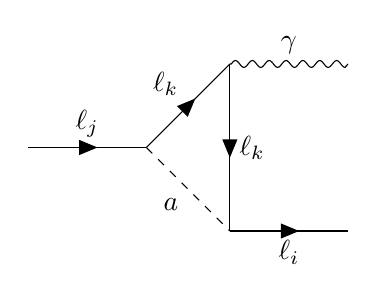
\begin{tikzpicture}[baseline=(current bounding box.center)]
    \begin{feynman}
        \vertex (b1);
        \vertex[right=of b1] (b2);
        \vertex[above right=of b2] (a3);
        \vertex[below right=of b2] (c3);
        \vertex[right=of a3] (a4);
        \vertex[right=of c3] (c4);
        \diagram* {
            (a3) -- [boson, edge label=\(\gamma\)] (a4),
            (b1) -- [fermion, edge label=\(\ell_j\)] (b2),
            (b2) -- [fermion, edge label=\(\ell_k\)] (a3),
            (b2) -- [scalar, edge label'=\(a\)] (c3),
            (a3) -- [fermion, edge label=\(\ell_k\)] (c3),
            (c3) -- [fermion, edge label'=\(\ell_i\)] (c4)
        };
    \end{feynman}
\end{tikzpicture}
    \caption{Lepton flavor-violating decay $\ell_j \to \ell_i \gamma$. The fermion running inside the loop is always the one not present in the initial and final states.}
    \label{fig:lep-decay}
\end{figure}

Turning our attention to the leptons, the decay width for a heavier lepton $\ell_j$ into a lighter one $\ell_i$ plus an on-shell photon is given by \cite{Cornella:2019uxs}
\begin{equation}\label{eq:lfv-decay}
    \Gamma (\ell_j \to \ell_i \gamma) = \frac{m_{\ell_j}}{8 \pi} e^2 \left( \abs{\mathcal{F}_{ij}(0)}^2 + \abs{\mathcal{G}_{ij}(0)}^2 \right) \,,
\end{equation}
where $m_j$ is the mass of the heavier lepton, $m_\mu$ or $m_\tau$. The Feynman diagram of these decays is depicted in Figure \ref{fig:lep-decay}. In the above equation, $\mathcal{F}_{ij}$ and $\mathcal{G}_{ij}$ are different functions for each case in hand. For the $\mu \to e \gamma$ decay,
\begin{equation}\label{eq:FandGemu}
    \begin{split}
        \mathcal{F}^{\mu e}_2(0)_{\text{quad}} &= -\frac{m_\mu m_\tau}{32 \pi^2 \Lambda^2} (a_{\tau \mu} a_{\tau e}  - v_{\tau \mu} v_{\tau e} ) g_3(x_\tau) \\
        \mathcal{G}^{\mu e}_2(0)_{\text{quad}} &= -\frac{m_\mu m_\tau}{32 \pi^2 \Lambda^2} (a_{\tau \mu} v_{\tau e}  - v_{\tau \mu} a_{\tau e}) g_3(x_\tau) \,.
    \end{split}
\end{equation}
where $a_{ji}$, $v_{ji}$ are the axial and vectorial LFV coupling constants connecting two leptons, $\ell_j$ and $\ell_i$, with the flavon, respectively. The variable $x_j$, $j=\mu, \tau$ is defined as
\begin{equation}
    x_j = \frac{m_j^2}{m_a^2}-i\eta,\; \eta\to 0^+ \,.
\end{equation}

For the $\tau \to \mu \gamma$ case, we have
\begin{equation}\label{eq:FandGeta}
    \begin{split}
        \mathcal{F}^{\tau \mu}_2(0)_{\text{quad}} &= -\frac{m_\mu m_\tau}{32 \pi^2 \Lambda^2} (a_{\tau e} a_{\mu e} + v_{\tau e} v_{\mu e}) g_4(x_\tau) \\
        \mathcal{G}^{\tau \mu}_2(0)_{\text{quad}} &= +\frac{m_\mu m_\tau}{32 \pi^2 \Lambda^2} (a_{\tau e} v_{\mu e} + v_{\tau e} a_{\mu e}
        ) g_4(x_\tau) \,.
    \end{split}
\end{equation}
There is also the $\tau \to \mu \gamma$ decay, where
\begin{equation}\label{eq:FandGmuta}
    \begin{split}
        \mathcal{F}^{\tau e}_2(0)_{\text{quad}} &= -\frac{m_\mu m_\tau}{32 \pi^2 \Lambda^2} (a_{\tau \mu} a_{\mu e} - v_{\tau \mu} v_{\mu e}) g_4(x_\tau) \\
        \mathcal{G}^{\tau e}_2(0)_{\text{quad}} &= -\frac{m_\mu m_\tau}{32 \pi^2 \Lambda^2} (a_{\tau \mu} v_{\mu e} - v_{\tau \mu} a_{\mu e}) g_4(x_\tau) \,.
    \end{split}
\end{equation}

\begin{figure}
    \centering
    \begin{tikzpicture}[baseline=(current bounding box.center)]
    \begin{feynman}
        \vertex (c1) {\(\ell_j\)};
        \vertex[right=of c1] (c2) ;
        \vertex[right=of c2] (c3);
        \vertex[right=of c3] (c4) {\(\ell_j\)};
        \vertex[above right=1.06cm of c2] (b);
        \vertex[below right=1.06cm of b] (x);
        \vertex[above=of b] (a) {\(\gamma\)};
        \diagram* {
            (c1) -- [fermion] (c2);
            (c2) -- [scalar, edge label'=\(a\)] (c3);
            (c3) -- [fermion] (c4);
            (c2) -- [fermion, edge label=\(\ell_k\)] (b);
            (b) -- [fermion, edge label=\(\ell_k\)] (x);
            (a) -- [boson] (b)
        };
    \end{feynman}
\end{tikzpicture}
    \caption{Feynman diagram of the main contribution to $(g-2)$ from lepton flavor-violating couplings.}
    \label{fig:g-2-tikz}
\end{figure}

The $(g-2)_{\ell}$ uncertainty limits are codified by our parameters through the expressions
\begin{equation}\label{eq:g-2}
    \begin{split}
        (\Delta a_e)_{\rm{LFV}} &=  \frac{m_e^2}{16 \pi^2 \Lambda^2} \left[ \frac{m_\mu}{m_e}\qty(\abs{v_{e\mu}}^2- \abs{a_{e\mu}}^2)g_3(x_\mu) + \frac{m_\tau}{m_e} \qty( \abs{v_{e \tau}}^2 - \abs{a_{e \tau}}^2)g_3(x_\tau)  \right] \\
        (\Delta a_\mu)_{\rm{LFV}} &= \frac{m_e^2}{16 \pi^2 \Lambda^2} \left[ \qty(\abs{v_{e\mu}}^2+ \abs{a_{e\mu}}^2)h_3(x_\mu) + \frac{m_\tau}{m_\mu} \qty( \abs{v_{\mu \tau}}^2 - \abs{a_{\mu \tau}}^2)g_3(x_\tau)  \right] \,.
    \end{split}
\end{equation}

The loop functions $g_3(x)$, $g_4(x)$, and $h_3(x)$ are
\begin{equation}
    \begin{split}
        g_3(x) &= \frac{2x^2 \ln x - (x-1)(3x-1)}{(x-1)^3} \\
        g_4(x) &= 1 - 2x + 2(x-1)x \ln \frac{x}{x-1} \\
        h_3(x) &= 2x^2 \ln \frac{x}{x-1} -1 -2x\,.
    \end{split}
\end{equation}

 \bibliography{myrefs}
\end{document}


